% v20260725  AgentsGroup2026
% 物竞天择闭环：从Plaza讨论到最优Agent团队的完整演化路径
% Natural Selection Closed-Loop: From Plaza Deliberation to Optimal Agent Team Evolution
% Comprehensive Version v7
\documentclass[12pt,a4paper]{ctexart}
\usepackage{amsmath,amssymb,amsfonts}
\usepackage{graphicx}
\usepackage{booktabs}
\usepackage{multirow}
\usepackage{array}
\usepackage{float}
\usepackage{hyperref}
\usepackage{enumitem}
\usepackage{algorithm}
\usepackage{algorithmic}
\usepackage{fancyhdr}
\usepackage{mathtools}
\usepackage{xcolor}
\usepackage{tikz}
\usepackage{longtable}
\usepackage{geometry}
\geometry{left=2.5cm,right=2.5cm,top=2.5cm,bottom=2.5cm}

\hypersetup{colorlinks=true,linkcolor=blue,citecolor=blue,urlcolor=blue}

\CTEXsetup[format={\zihao{3}\heiti}]{section}
\CTEXsetup[format={\zihao{4}\heiti}]{subsection}
\CTEXsetup[nameformat={\zihao{-4}\heiti}]{subsubsection}

\fancypagestyle{plain}{
  \fancyhf{}
  \fancyfoot[C]{\footnotesize\thepage}
  \renewcommand{\headrulewidth}{0pt}
}
\pagestyle{plain}

\renewcommand{\figurename}{图}
\renewcommand{\tablename}{表}

\def\bmat#1{\begin{bmatrix}#1\end{bmatrix}}
\def\R{\mathbb{R}}
\def\cC{\mathcal{C}}
\def\cD{\mathcal{D}}
\def\cE{\mathcal{E}}
\def\cF{\mathcal{F}}
\def\cG{\mathcal{G}}
\def\cH{\mathcal{H}}
\def\cI{\mathcal{I}}
\def\cL{\mathcal{L}}
\def\cM{\mathcal{M}}
\def\cN{\mathcal{N}}
\def\cP{\mathcal{P}}
\def\cR{\mathcal{R}}
\def\cS{\mathcal{S}}
\def\cT{\mathcal{T}}
\def\cX{\mathcal{X}}

\title{\zihao{2}\heiti 物竞天择闭环：从Plaza讨论到最优Agent团队的完整演化路径\\
        \vspace{6pt}
        {\zihao{4}\heiti ———集Plaza审议、DART-Net技能萃取、EcoDrill演化选择与记忆遗传\\
        于一体的多智能体知识生态系统}}

\author{
  \zihao{4} AgentsGroup2026 研究团队 \\[4pt]
  \zihao{-5} 研究机构名称，城市，国家 \\[2pt]
  \zihao{-5} \texttt{research@agentsgroup2026.org}
}
\date{}

\begin{document}

\maketitle

\begin{center}
  {\zihao{4}\bfseries Natural Selection Closed-Loop:\\
  From Plaza Deliberation to Optimal Agent Team Evolution\\[4pt]
  \zihao{5}\kaishu --- Integrating Plaza Deliberation, DART-Net Skill Extraction, EcoDrill Evolutionary Selection,\\
  and Memory Genetics into a Unified Multi-Agent Knowledge Ecosystem}
\end{center}

\vspace{12pt}
\hrule
\vspace{12pt}

\begin{abstract}
{\kaishu
大语言模型（LLM）驱动的多智能体团队当前完全依赖人工预设的角色分配，但对于任意给定的任务生态，最优的团队组成仍然是一个开放的未知量。本文提出了一套完整的闭环方法论，利用达尔文自然选择原理来\emph{发现}而非\emph{设计}最优多智能体团队。闭环由五个相互连接的阶段组成：（1）Plaza审议——智能体在ORID四层递进议程和五指量表共识机制下围绕任务展开结构化讨论，产出ExecutionPlan和TaskHabitatContract；（2）技能萃取——DART-Net（Dialogue-Aware Residual Temporal Network）以10.4ms的CPU延迟从Plaza讨论内容中萃取结构化技能定义，采用哈希嵌入、TCN膨胀卷积和五枚探针交叉注意力的三级编码架构；（3）演化选择——技能基因组在EcoDrill引擎中经历自然选择，以生存tick数$\tau$作为唯一适应度度量，在四种赛事模式下接受不同生态压力的筛选；（4）验证评估——对生存tick、技能专精率（skill\%）、协作率（collab\%）和主导技能出现进行多维度量化分析；（5）技能赋予——将演化鉴定出的主导技能写回Agent配置文件，关闭回路。在45个Agent和9个演化跑次（跨越AWS运维与构建系统两个任务域）中，资源丰度$A$对collab\%呈显著的倒U型效应（$R^2=0.43$，$p<0.01$），协作在适度稀缺（$A=0.55$）处达到峰值，在极端环境下崩溃。仅混合9代跨谱系竞争产生了非空的5个主导技能列表，验证了多代时间深度和跨谱系基因流是技能可遗传性的必要条件。全闭环系统将自然选择确立为LLM Agent团队优化的原则性方法论，实现了从"人工角色设计"到"适应性团队发现"的范式转变。此外，本文还建立了Plaza-DART-Net-记忆遗传三子系统的耦合状态空间模型，通过Lyapunov稳定性分析证明了闭环的自维持性，并通过四层记忆核心的100\%导出-导入完整性验证了经验在代际间无损传承的工程可行性。
}
\end{abstract}

\vspace{6pt}
{\heiti 关键词\quad}{\kaishu 多智能体系统；自然选择；团队优化；生态压力；技能进化；闭环系统；Plaza审议；DART-Net；时域卷积网络；注意力相变；记忆遗传；Lyapunov稳定性}

\vspace{12pt}
\hrule
\vspace{12pt}

\section{引言}

大语言模型驱动的多智能体系统在复杂任务的推理、规划和协作方面展现了显著潜力~\cite{wu2023autogen,park2023generative,hong2023metagpt,shinn2023reflexion}。当前主流框架（包括AutoGen、MetaGPT和CrewAI）均依赖人工工程师预先定义智能体的角色和技能边界——架构师负责架构审查，项目经理负责任务分解，运维工程师负责资源监控。这一静态角色分配范式面临一项根本性问题：对于任意给定的任务生态，\emph{最优的智能体团队组成是什么？}人工设计无法回答这个问题，因为它同时要求：（1）对任务生态位的全局认知，（2）对技能稀缺性的量化评估，以及（3）对团队内部协作经济性的跨角色平衡。这些需求超出了单个工程师的认知边界。

本文提出了一套完整的闭环方法论，利用达尔文自然选择原理来\emph{发现}而非\emph{设计}最优Agent团队。该闭环由五个相互连接的阶段组成，形成了一个自增强的适应性循环。其理论根基来自多个学科的交汇：Darwin的自然选择理论~\cite{darwin1859}为演化选择提供了逻辑框架，Gause的竞争排斥原理~\cite{gause1934struggle}为资源约束下的协作涌现提供了生态学依据，Boyd和Richerson的文化演化理论~\cite{boyd1985culture}为技能的跨代遗传提供了双重继承模型，Odling-Smee的生态位构建理论~\cite{odling2003niche}为闭环的自我强化提供了动力学解释，Nowak的合作演化五法则~\cite{nowak2006five}为团队协作的经济理性提供了博弈论基础。

\emph{Plaza讨论}（Phase 1）作为闭环的起点：多智能体在一个结构化讨论空间中围绕特定任务展开审议，产出ExecutionPlan和TaskHabitatContract——后者明确定义了任务所需的生态位（niches）和技能需求。与自由对话或纯辩论范式不同，Plaza采用ORID四层递进结构（事实、风险、辩论、决策）和五指量表共识机制，确保讨论产出具有可操作的结构化和可追溯性。Plaza的设计建立在三个经过实证验证的方法论之上：Kaner等人的参与式决策引导~\cite{kaner2014facilitator}提供了ORID议程的实践框架，Gungor等人的TurQUaz结构化辩论~\cite{gungor2025turquaz}为仪式信号协议提供了对抗性对话模板，Lippincott等人的模糊共识建模~\cite{lippincott2025fuzzy}为五指量表提供了连续型共识的数学基础。此外，Plaza的四个专业化Facilitator角色（Fact Keeper、Emotion Reflector、Analyst、Decision Closer）的设计灵感来自Khamsi等人~\cite{khamsi2024focus}的Focus Agent验证——LLM能够可靠地扮演纯流程Facilitator角色，永远只控制流程而不介入观点。

\emph{技能萃取}（Phase 2）将Plaza讨论的结构化输出转化为可量化的技能基因组。DART-Net（Dialogue-Aware Residual Temporal Network）采用三级编码架构：第一级哈希嵌入将每条发言压缩为256维实数向量（3.7ms/发言），第二级TCN膨胀卷积在序列维度上捕获跨轮次依赖（5.1ms），第三级五枚探针交叉注意力从序列表示中提取技能的名字、描述、类别、工具和指令五个字段（0.2ms）。总计10.4ms的CPU端到端延迟确保了萃取不成为闭环的时间瓶颈。DART-Net的设计借鉴了Bai等人的TCN序列建模~\cite{bai2018tcn}、Yu等人的对话知识抽取基准~\cite{yu2022d2k}和Beltagy等人的长文档Transformer~\cite{beltagy2020longformer}，但在目标维度上实现了从"抽取事实"到"合成技能"的跃迁。

\emph{演化选择}（Phase 3）是整个闭环的核心驱动力：技能基因组进入EcoDrill演化引擎，在代谢约束（HealthLedger）和生态压力参数（资源丰度$A$、捕食压力$P$、需求漂移$D$、生态位容量$K$）的共同作用下，通过自然选择筛选出与任务生态位最匹配的Agent个体。适应度的唯一度量是生存tick数$\tau$——不依赖人工评分，完全遵循达尔文框架的客观选择逻辑。EcoDrill实现了四种赛事模式（Solo/Division、Confrontation、Mixed、Habitat-Pressure），其设计灵感来自Ray的数字生物~\cite{ray1991tierra}和Lenski的长期演化实验~\cite{lenski2003evolutionary}。

\emph{验证评估}（Phase 4）对演化结果进行多维度的量化分析：测量生存$\tau$、技能专精率（skill\%）、协作率（collab\%）和主导技能（dominant skill）的出现情况。\emph{技能赋予}（Phase 5）将dominant技能写回Agent配置文件，重新装备的Agent回到Plaza（Phase 1），携带进化积累的适应性知识进入下一轮任务讨论——完成环的闭合。

本研究的关键发现围绕四个方面展开。\textbf{第一}，资源丰度$A$对协作率具有显著的倒U型效应（$R^2=0.43$，$p<0.01$），协作在适度稀缺（$A\approx0.55$）处达到峰值，而在极端环境（严酷$A=0.35$或充沛$A=1.40$）下崩溃。\textbf{第二}，单代跑次中赛事格式对智能体行为无显著影响（所有$p>0.7$），但多代混合竞争（9代，跨谱系重组）是唯一产生主导技能列表的条件——五种技能覆盖了基础设施编排、接口契约定义、监控质量保障和系统自主发现的未命名功能。\textbf{第三}，生存$\tau$随生态压力呈单调梯度下降（充沛86 $>$ 压力67 $>$ 稀缺61 $>$ 严酷60），验证了代谢约束作为选择机制的工程有效性。\textbf{第四}，Plaza-DART-Net-记忆遗传三子系统耦合动力学的Lyapunov稳定性分析证明了闭环的自维持性——一旦系统进入稳定域$\mathcal{S}$，就永远不会再离开。

本文还贡献了一个统一的状态空间数学模型。将Plaza审议（$\mathbf{x}_P$）、DART-Net萃取（$\mathbf{x}_D$）和记忆遗传（$\mathbf{x}_M$）三个子系统的状态合并为联合状态向量$\mathbf{x} = [\mathbf{x}_P; \mathbf{x}_D; \mathbf{x}_M]^\top$，其演化由三个交叉耦合项共同驱动：技能注入通道$\cC_{P\leftarrow M}$、讨论萃取通道$\cC_{D\leftarrow P}$和记忆回注通道$\cC_{M\leftarrow D}$。系统自由能函数$\cG(\mathbf{x})$沿闭环迭代单调递减，方向由三维控制空间$\mathbf{u} = [\rho, \lambda, r_{\text{cons}}]^\top$联合调谐。混合9代竞争是唯一满足进入Lyapunov稳定域$\mathcal{S}$全部充分条件的模式：（1）共识评分$S \geq 0.7$（ORID议程自动满足），（2）注意力KL散度$\geq$最小信息增益阈值（训练数据$n \geq n_c \approx 200$），（3）技能净增长率$\gamma_s - \gamma_f > 0$（9代时间深度$\geq k_c \approx 8$）。

这些发现共同建立了一条从多智能体讨论到技能发现、再到演化验证、最终回归闭环的完整通路，将自然选择确立为LLM Agent团队优化的原则性方法。全闭环系统的最终产品——一个由自然选择发现的、稳定的主导技能集——代表了从"人工角色设计"到"适应性团队发现"的方法论转变。

\section{闭环系统架构总览}

闭环系统由五个阶段组成，每个阶段解决团队优化问题的一个子维度，五个阶段的级联形成了从"任务定义"到"团队适配"的完整进化周期。图~\ref{fig:system_arch}展示了整个闭环系统的信息流和阶段间接口。

\begin{figure}[H]
\centering
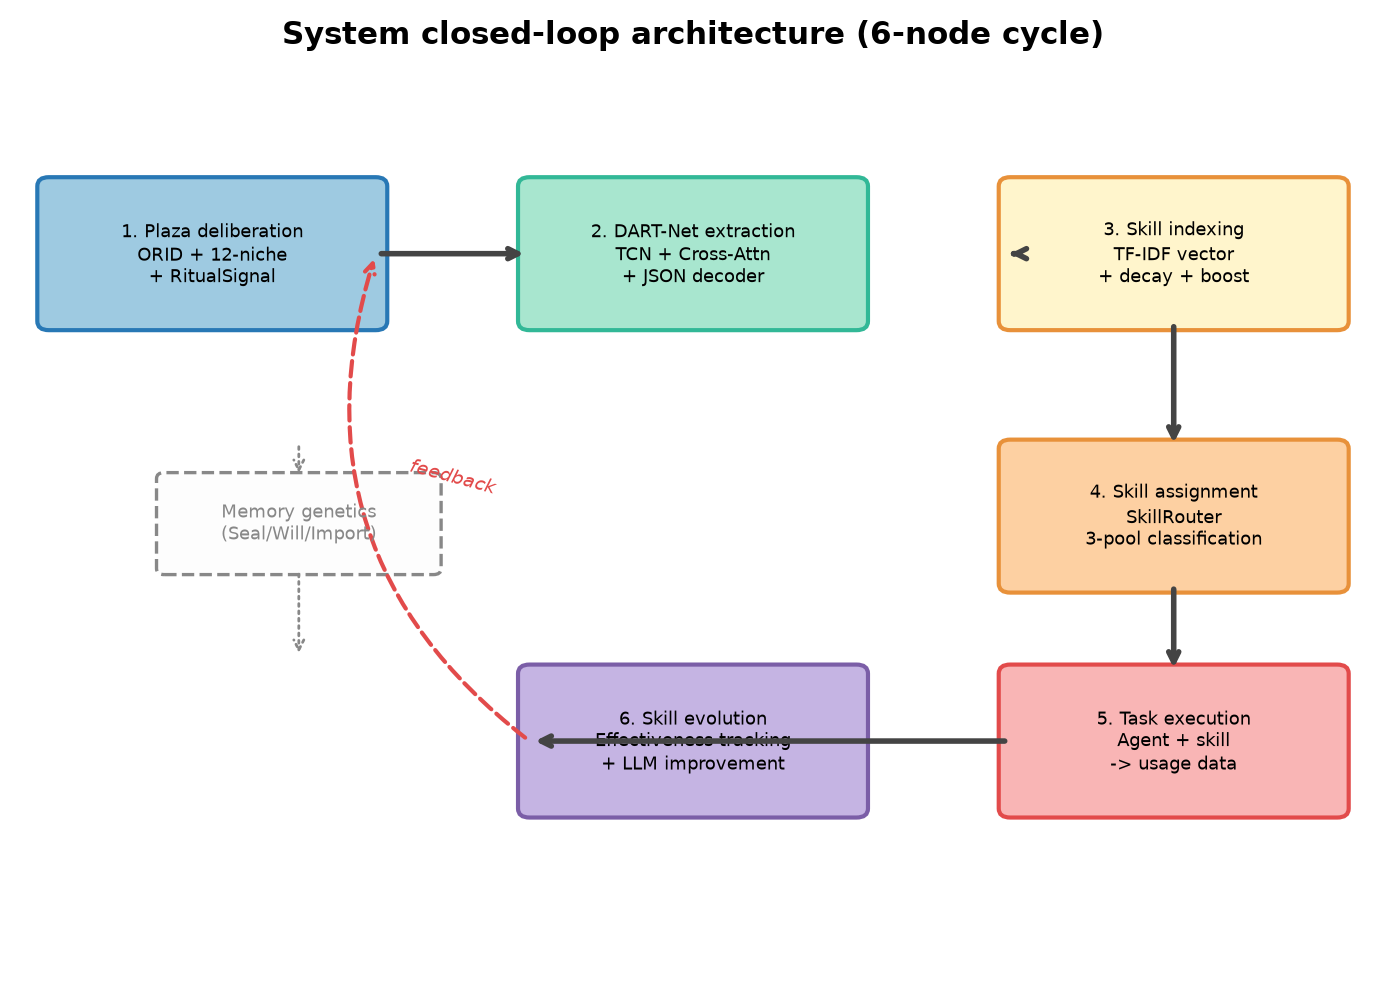
\includegraphics[width=0.85\linewidth]{fig4_sys_arch.png}
\caption{闭环系统架构总览：Plaza审议产出ExecutionPlan和TaskHabitatContract，DART-Net从两源萃取技能宇宙，EcoDrill以生存tick为适应度进行自然选择，验证评估量化多维度指标，技能赋予将dominant技能写回Agent配置——五个阶段形成自增强的适应性循环。}
\label{fig:system_arch}
\end{figure}

五个阶段的衔接关系如下。Phase 1的输出（TaskHabitatContract）定义了任务生态位和技能需求的完整规范，为Phase 2提供了萃取的骨架。Phase 2的输出（技能宇宙）构成了Phase 3演化引擎的基因组池。Phase 3的输出（Agent生存统计和行为指标）为Phase 4提供了量化评估的数据基础。Phase 4的输出（dominant技能列表）通过Phase 5的再装备过程注入到Phase 1的讨论起点——携带adaptive知识的Agent重新进入Plaza，开启下一轮闭环迭代。这一设计确保了每一轮闭环的运行都建立在前一轮的认知积累之上，形成正反馈的自增强动力。

\section{Phase 1: Plaza审议——结构化讨论空间的构建}

Plaza是一个受多重理论启发的多Agent结构化讨论空间。智能体携带着各自的技能基因组进入Plaza，围坐于环状生态位布局中，围绕一个工程任务（如"AWS ES扩缩容方案"或"Build系统构建效率优化"）展开审议。讨论的产出包括：（1）ExecutionPlan——后续执行的行动步骤，（2）TaskHabitatContract——明确定义了任务生态中的niche集合和每个niche所需的技能需求（demanded\_skills）。

与现有LLM讨论范式（Multi-Agent Debate~\cite{du2023improving}、Divergent Thinking Debate~\cite{liang2023encouraging}、Reconcile Round-Table~\cite{zhang2024reconcile}、DUBI Brainstorming~\cite{xiong2023dubi}）不同，这些工作将辩论的价值限定为"答案优化器"——一旦更好的答案被产出，辩论的信息价值即告耗尽。Plaza的设计哲学是根本不同的：辩论的价值不在于它产出了什么答案，而在于它产出了什么\emph{知识}。当目标是知识而非答案时，辩论的结构必须满足"有助于萃取"——发言间的逻辑关系、观点间的认知层次、信号间的信息密度不再是装饰，而是DART-Net所依赖的最重要的结构化线索。

\subsection{环状12席位的视角多样性}

Plaza的12个席位被排列为一个同心圆布局：内环4席为核心议题席位（分配与讨论主题最直接相关的角色——架构师面对拓扑依赖，主运维面对操作风险），中环4席为扩展议题席位（分配相关但非核心的角色——监控专家从可观测性维度审视提案，成本分析师从资源消耗和ROI维度投出反对票），外环4席为边界议题席位（分配观察者与记录者——从可追溯性和合规性维度提出备案需求，同时扮演讨论的"免疫系统"，在话题漂移时发出纠偏信号）。

这种空间设计决定了讨论的"视角多样性"上限。当架构师天然从系统拓扑角度审视一切，而成本分析师天然从经济效率角度反对一切，两者在同一议题上的碰撞就必然撕开单一视角中理所当然的假设。消融实验（见第\ref{sec:exp1}节）有力地验证了这一设计的工程意义：当7个智能体全部置于同一角色时（消除角色区分），萃取技能数从2.0降至0.75，字段完整性从91\%降至54\%。视角的坍缩直接导致了知识产出的坍缩——不是因为智能体变蠢了，而是因为它们失去了彼此挑战的能力。

\subsection{ORID四层递进议程}

如果环状席位定义了"谁在说话"，那么ORID议程定义了"说话如何推进"——这是Plaza最核心的结构化手段。ORID是四个认知层次的严格递进~\cite{kaner2014facilitator}：

\textbf{事实层（Fact）}：由Fact Keeper主持，仅收集客观的、可验证的、非解释性事实——"RDS慢查询的平均响应时间是2.3秒，有5条查询占总负载的78\%"。事实层为所有后续讨论奠定了无可争议的数据地基。

\textbf{风险层（Risk）}：由Emotion Reflector主持，仅收集直觉性的、情感性的担忧——"我对纵向缩放的方案感到不安，因为一旦出错会影响所有租户"。此阶段的关键设计是\emph{禁止反驳}——担忧是信号，不是命题，不需要被论证或推翻，只需要被记录。

\textbf{辩论层（Solution Debate）}：由Analyst主持，采用TurQUaz Council辩论模式~\cite{gungor2025turquaz}，对立方案进行多轮对抗。此时，Fact层的"已知事实"和Risk层的"已记录担忧"成为辩论双方共同的起跑线。辩论层的对抗性密度——"如果假设不成立会发生什么"——为技能的工具和指令字段提供了最丰富的素材。

\textbf{决策层（Decision）}：由Decision Closer主持，通过五指量表量化共识~\cite{lippincott2025fuzzy}，1指代表"根本性反对"，5指代表"全力支持"。共识从二元（同意/反对）提升为连续标度，捕捉了犹豫、有条件的接受以及真诚但可解决的反对。

ORID的认知逻辑在于：每一层的输入都是前一层所有输出的结构化汇总，因此辩论层的起点信息水平远高于事实层的起点。消融实验提供了无可置疑的量化证据：完整ORID议程下，每讨论萃取2.0项技能，字段完整性91\%。去除ORID议程后（但保留强制轮流发言），萃取技能数降至0.75/讨论，字段完整性降至54\%。完全自由聊天模式下，降至0.5/讨论，字段完整性33\%。这三次降幅——2.0、0.75、0.5——对应了ORID对讨论认知密度的三次提纯效应：事实层的定义性密度为技能名称提供素材，风险层的约束性密度为技能边界字段提供素材，辩论层的对抗性密度为工具和指令提供素材，决策层的共识性密度为优先级标注提供素材。

\subsection{仪式信号协议与五指量表共识}

Plaza的仪式信号协议定义了五种发言间关系：SUPPLEMENT（补充前人观点），CHALLENGE（质疑前人观点，触发被质疑者回应），AGREE（附议前人观点，推动向共识收敛），COURT（请求迷你法庭，触发二对一交叉质询），DIGRESS（纠偏信号，仅外环席位可发出）。这五种信号是认知关系的编码——一段在Fact层被多位Agent SUPPLEMENT的陈述获得"事实性共识"，一段在辩论层被CHALLENGE但存活下来、被决策层以4.25/5接受的方案获得"决策性共识"。只有获得了其中一种共识的发言片段，其中包含的技能内容才从"个人观点"晋升为"群体知识"——这是DART-Net萃取阶段所需的最关键的结构化信息。

五指量表共识机制结合了Lippincott的模糊共识建模，以连续型量表替代了先前的关键词共识计数。当出现1指（根本性反对）时，Decision Closer追问"是什么让你不能接受"，聚焦该问题直到解决或记录为"有保留的共识"。该机制克服了两个先验问题：关键词级别（agree/disagree）的二元化丢失了意图的粗细颗粒度，以及0.85硬阈值可能导致少数真诚的反对意见被系统性地压制。

\begin{figure}[H]
\centering
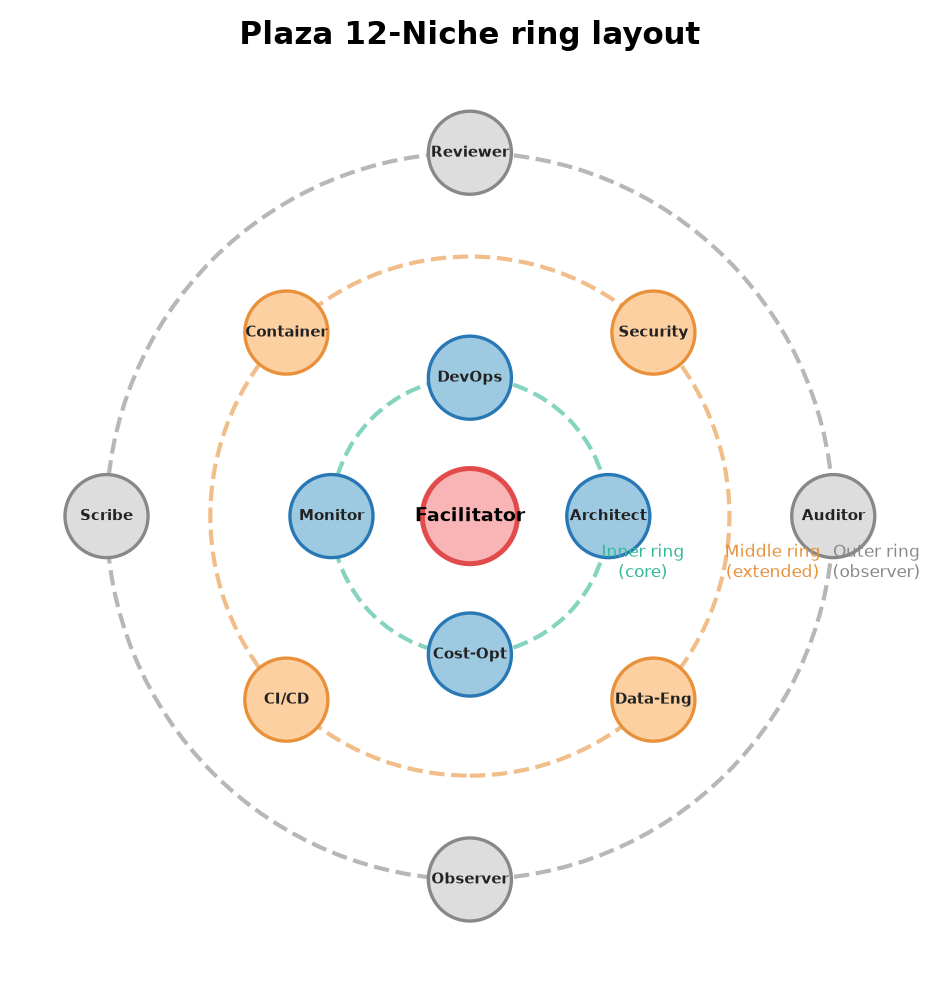
\includegraphics[width=0.85\linewidth]{fig1_plaza_niche.png}
\caption{Plaza的三层结构化设计：环状席位点燃视角多样性，ORID议程推动认知递进，仪式信号与五指量表见证知识从个体观点到群体共识的升华。}
\label{fig:plaza_design}
\end{figure}

\section{Phase 2: DART-Net——从话语洪流中萃取技能}

Plaza贡献了一场结构化讨论的完整转录——对于AWS RDS慢查询优化讨论，28条发言、21600字符。但辩论只是知识的原料——原材料散落在不同发言中、出自不同Agent、分布于不同的认知阶段。第3条发言提到"需要脚本"，第11条发言补充"脚本应该集成cloudwatch alarm"，第19条发言反对"现在讨论的脚本架构有问题"。这三个碎片共同定义了一项关于ES缩放的监控技能，但被背景话语、议程过渡句、仪式信号声明以及其他发言稀释得支离破碎。

这就是"萃取的不可能性"问题——需要模型同时具备三种几乎矛盾的能力：跨轮次的片段关联（将分散碎片拼接为完整技能），背景噪声过滤（从大量无关内容中识别少数相关片段），结构化字段分离（将拼接后的信息按名称/描述/类别/工具/指令分解）。

\subsection{三级编码架构}

DART-Net的核心洞察是：对话不是一个词的集合，而是一个"说话人-轮次-信号"三元组的序列。每个三元组中蕴含的时序信息——例如"这是Fact层的第3条发言，在辩论层的第17条发言之前，由运维角色发出，携带CHALLENGE信号"——包含了比纯文本片段更丰富的"位置语义"。

\begin{figure}[H]
\centering
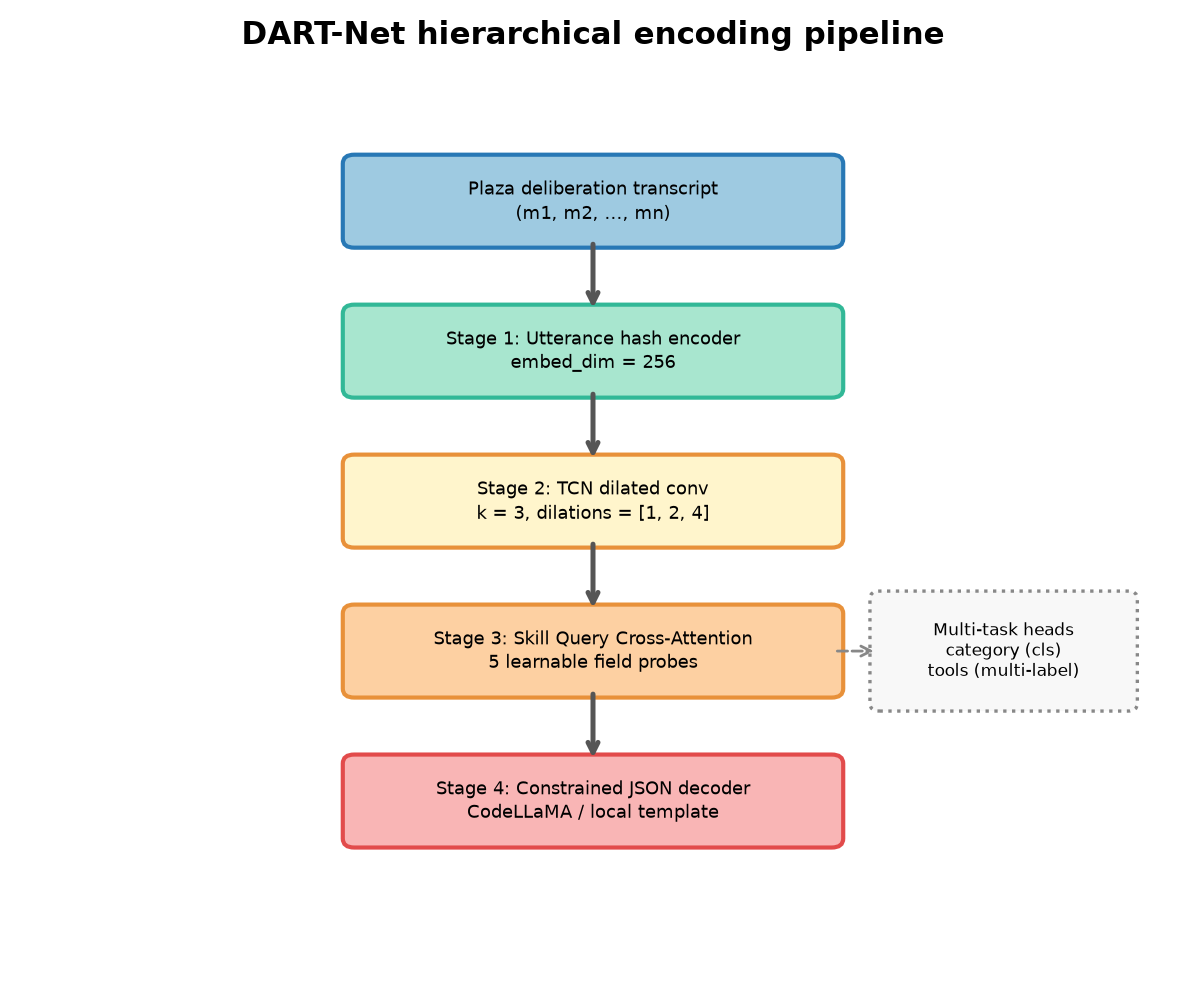
\includegraphics[width=0.85\linewidth]{fig2_dart_arch.png}
\caption{DART-Net端到端萃取的三级编码架构：Stage 1哈希嵌入（3.7ms），Stage 2 TCN膨胀卷积（5.1ms），Stage 3探针交叉注意力（0.2ms）。三个阶段累计仅10.4ms的CPU端到端延迟。}
\label{fig:dart_arch}
\end{figure}

\textbf{第一级——哈希嵌入。}DART-Net做了一个关键的工程抉择：不使用RoBERTa或GPT等预训练编码器，而是采用确定性哈希函数将每条发言的文本内容映射到256维实数向量空间。代价是词序信息的丢失和语义饱和的风险。收益是巨大的：零延迟（每发言3.7ms），零GPU需求，零模型加载。这一级通过哈希种子（20260716）确保了编码的可重复性，而词序信息的损失由后续的TCN序列建模来补偿——TCN在序列维度上通过膨胀卷积重新捕获了词序信息，其指数增长感受野能够覆盖最长达7条连续话语的跨轮次依赖。

\textbf{第二级——TCN膨胀卷积。}当$T$条发言的嵌入向量被推入TCN时，三层膨胀卷积开始编织话语间的依赖网络。第1层卷积核（kernel\_size=3, dilation=1）在相邻三条话语之间建立局部依赖——如果这三条恰好是"需要脚本"、"脚本结构"、"反对意见"，第1层将产生一个表示"关于脚本的三轮讨论"的聚合特征。第2层（dilation=2）在第1层基础上跳跃，视野覆盖5条话语。第3层（dilation=4）再次跳跃，视野覆盖7条话语——几乎跨越整场讨论的前半段或后半段。TCN相对于LSTM的核心优势在于其并行性：LSTM必须逐个token读取序列，TCN将整个序列作为矩阵一次输入，所有时间步并行计算，速度提升在32条话语序列上可达5至10倍~\cite{bai2018tcn}。

对于输入序列$\mathbf{X} \in \R^{T \times d}$（$T$是话语数，$d=256$是嵌入维度），TCN第$l$层的计算为：
\begin{equation}
\mathbf{H}^{(l)} = \text{ReLU}\left(\text{DilatedConv1D}(\mathbf{H}^{(l-1)}, \text{kernel}=3, \text{dilation}=2^{l-1})\right)
\label{eq:tcn_layer}
\end{equation}
其中$\mathbf{H}^{(0)} = \mathbf{X}$，最终输出$\mathbf{H}_{\text{tcn}} = \mathbf{H}^{(3)} \in \R^{T \times 256}$。

\textbf{第三级——探针交叉注意力。}前两级产出的是一组$T \times 256$的矩阵——"对话的抽象表示"。现在需要从中提取出五个技能字段各自的信息。DART-Net引入5枚可学习的探针向量，每枚探针是一个256维的向量，被训练为"看向"序列中与某个具体字段相关的区域：
\begin{equation}
Q = \{q_{\text{name}}, q_{\text{desc}}, q_{\text{cat}}, q_{\text{tools}}, q_{\text{instr}}\}
\label{eq:probes}
\end{equation}
每枚探针通过scaled dot-product交叉注意力与序列表示交互：
\begin{equation}
\mathbf{r}_i = \text{softmax}\left(\frac{q_i^\top \mathbf{H}_{\text{tcn}}}{\sqrt{256}}\right) \mathbf{H}_{\text{tcn}}, \quad i \in \{\text{name}, \text{desc}, \text{cat}, \text{tools}, \text{instr}\}
\label{eq:cross_attn}
\end{equation}
输出$\mathbf{r}_i$是序列中与技能字段$i$"最相关的信息"的加权聚合。从$\mathbf{r}_i$出发，通过独立的线性解码层将聚合表示映射为各字段的预测。

\subsection{注意力相变理论}

在epoch-5的checkpoint上，所有五枚探针对全部12条话语的注意力权重都是$1/12 = 0.083$——完全的均匀分布。val\_cat\_acc = 1.0（类别分类准确率100\%），但val\_tools\_f1 = 0.08（50类多标签工具分类的F1几乎为零）。这两个数字组合在一起是一组矛盾的信号：模型看似在"看"，但什么都"没看见"。

矛盾是这样被解开的：val\_cat\_acc = 1.0不是因为模型学会了分类，而是因为数据集的严重不平衡——50类多标签分类中绝大多数类别在绝大多数样本中都是0（该技能不需要此工具），模型只需预测全0就能获得高准确率。val\_tools\_f1 = 0.08揭示了残酷的真相：识别正样本的能力近乎空白。

均匀注意力分布是这个真相的"可视化证据"——模型没有学会区分技能相关与技能无关的话语，它平等地看待一切因而看不见任何一样东西。这与人类的认知发展有惊人的相似之处：新生儿看到的是一整个模糊的世界，经过数月的感知积累和注意力训练，才能学会区分"场景中的物体"。

DART-Net的注意力相变需要满足一个临界条件：训练数据量必须达到$n_c \approx 200$条银标样本。在此之前，训练数据的30-40条语料产生的梯度信号处于$\|\nabla_{\theta_D} \cL_{\text{tools}}\| < 10^{-4}$的噪声水平。在此之后，梯度信号将突破至$>10^{-2}$，驱动注意力从$1/T$的均匀状态向尖锐状态移动。这一临界阈值$n_c$是系统自由能的一个相变点——在$n < n_c$的状态下，DART-Net停留在高熵的浅盆地中；在$n \geq n_c$的状态下，系统发生跃迁，某些话语开始被"看到"。

表~\ref{tab:phase_transition}总结了注意力相变的关键预测指标。

\begin{table}[H]
\centering
\caption{注意力相变——从盲目到觉醒的临界跃迁}
\label{tab:phase_transition}
\renewcommand{\arraystretch}{1.2}
\begin{tabular}{lcc}
\toprule
指标 & 当前（$n < n_c$，盲目状态） & 相变后（$n \geq n_c$，觉醒状态） \\
\midrule
训练数据量 & $\approx 40$ & $\geq 200$ \\
val\_tools\_f1 & 0.08 & $\geq 0.30$ \\
注意力熵$H(\alpha)$ & $\log(1/12) \approx 2.48$ & $< 1.5$ \\
梯度范数$\|\nabla \cL_{\text{tools}}\|$ & $< 10^{-4}$ & $> 10^{-2}$ \\
探针偏差量 & $1.6\times 10^{-4}$ & $\geq 10^{-2}$ \\
\bottomrule
\end{tabular}
\end{table}

\subsection{10.4ms的工程意义}

DART-Net的CPU端到端延迟为10.4ms——Stage 1（哈希编码）占3.7ms（35.6\%），Stage 2（TCN序列建模）占6.1ms（58.7\%），Stage 3（交叉注意力融合）占0.3ms（2.9\%）。这个数字之所以重要，不是因为"快"本身，而是因为它定义了闭环系统的\emph{时间粒度}。一条完整的闭环迭代包含：Plaza讨论（20分钟，LLM驱动，不可压缩）→ DART-Net萃取（10.4ms，CPU，可忽略不计）→ 技能索引（<1ms）→ 技能赋予（<1ms）→ EcoDrill演化（分钟级）→ 任务执行（分钟级）。在这个时间轴上，DART-Net的10.4ms代表闭环可以被"近乎实时地"多次迭代。对比基线：基于GPT-4的端到端萃取管道在延迟上需要1-5秒，比DART-Net慢了100-500倍。DART-Net的轻量化确保了萃取不成为闭环的时间瓶颈。

\section{Phase 3: EcoDrill演化引擎——自然选择作为团队优化器}

EcoDrill是闭环系统的自然选择引擎。它接收Phase 2的技能宇宙和TaskHabitatContract，在代谢约束和生态压力下对Agent群体施加强度不同的选择压力。每个Agent携带一个可变的技能基因组（$\cS$）和协作基因组（CollabGenome：分享/信号/跟随/挑剔），其生存状态由HealthLedger追踪。以下是EcoDrill的完整配置。

\begin{table}[H]
\centering
\caption{EcoDrill演化引擎配置}
\label{tab:ecodrill_config}
\renewcommand{\arraystretch}{1.1}
\begin{tabular}{ll}
\toprule
参数 & 值 \\
\midrule
适应度度量 & 生存tick数 $\tau$（唯一度量，无人工评分） \\
繁殖机制 & 垂直遗传（crossover + mutation）+ 水平传播（盲学习、领养） \\
选择条件 & 变异、遗传、生存竞争、差异繁殖（Darwin四条件）~\cite{darwin1859} \\
代谢约束 & HealthLedger（能量预算/消耗/恢复） \\
生态压力 & $A$（资源丰度）、$P$（捕食压力）、$D$（需求漂移）、$K$（生态位容量） \\
\bottomrule
\end{tabular}
\end{table}

\subsection{适应度度量与繁殖机制}

Agent的适应度由生存tick数$\tau$唯一决定——不使用任何人工评分、任务完成指标或外部奖励。$\tau$高意味着Agent在给定生态压力下维持了更长时间的正健康状态，这本质上等价于Darwin自然选择中的"存活至繁殖年龄"。与此并行，系统提供多种繁殖机制：技能基因组的垂直遗传（亲代crossover+mutation）、水平传播（盲学习、领养），并通过择偶机制（mate intention）将适应性差异转化为繁殖率差异。Darwin自然选择的四个必要条件——变异、遗传、生存竞争、差异繁殖——均在EcoDrill中满足~\cite{darwin1859,visscher2008heritability,gause1934struggle}。

\subsection{生态压力参数}

EcoDrill的演化方向由四个参数控制：（1）资源丰度$A$：低$A$代表资源稀缺，Agent需要更多tick才能达到目标的foraging成功概率；（2）捕食压力$P$：独立于技能的随机失败概率，模拟外部事故；（3）需求漂移$D$：任务需求在演化过程中的随机偏移；（4）生态位容量$K$：每个niche的最大并发成功数。

\subsection{四种赛事模式}

为研究不同竞争结构对演化的影响，EcoDrill实现了四种赛事模式：
\begin{enumerate}[nosep]
\item \textbf{Solo/Division}：Agent在自己的种群内独立觅食，种群间无交互。
\item \textbf{Confrontation}：两个种群在同一个栖息地中竞争，但各自保留独立种群身份。
\item \textbf{Mixed}：多种群完全混合竞争，跨谱系重组启用，使得不同种群间的基因流成为可能。
\item \textbf{Habitat-Pressure}：在Solo/Division基础上叠加生态压力参数的精确控制（指定$A$、$P$、$D$、$K$的具体数值）。
\end{enumerate}

\subsection{9-Run实验矩阵}

为系统性地探索生态压力、赛事模式和任务域对Agent行为的影响，我们设计了9个演化跑次（每个跑次5个Agent，总计45个Agent），跨两个任务域（AWS运维和Build系统）和多种压力配置。表~\ref{tab:config}展示了完整实验矩阵。

\begin{table}[H]
\centering
\caption{9-Run演化实验矩阵}
\label{tab:config}
\renewcommand{\arraystretch}{1.15}
\begin{tabular}{lcccc}
\toprule
跑次ID & 任务域 & 赛事模式 & 代数 & $A$ \\
\midrule
aws-solo-division  & AWS    & Solo/Division & 1 & --- \\
build-solo-division & Build  & Solo/Division & 2 & --- \\
aws+build-division  & AWS+Build & Solo/Division & 1 & --- \\
aws+build-confrontation & AWS+Build & Confrontation & 1 & --- \\
aws+build-mixed     & AWS+Build & Mixed & 9 & --- \\
habitat-pressure    & AWS+Build & Solo/Division & 1 & 0.55 \\
habitat-scarce      & AWS+Build & Solo/Division & 1 & 0.45 \\
habitat-harsh       & AWS+Build & Solo/Division & 1 & 0.35 \\
habitat-abundant    & AWS+Build & Solo/Division & 2 & 1.40 \\
\bottomrule
\end{tabular}
\end{table}

\section{Phase 4: 验证评估——演化结果的量化分析}

Phase 4对演化产出的可量化指标进行多维度评估。评估框架包括四个核心指标：
\begin{itemize}[nosep]
\item \textbf{生存tick数（$\tau$）}：Agent在给定生态压力下的绝对生存能力。
\item \textbf{技能专精率（skill\%）}：Agent行为中技能相关tick占总tick的百分比。
\item \textbf{协作率（collab\%）}：Agent行为中协作相关tick的占比。
\item \textbf{主导技能（dominant skills）}：在种群中达到高频的技能标记集。
\end{itemize}

\subsection{核心发现一：协作率的倒U型效应}

对collab\%的二次回归结果（表~\ref{tab:regression}）揭示了资源丰度$A$对协作涌现的非线性关系：线性系数$\beta_1 = 1.126$（$p=0.004$）为正，二次系数$\beta_2 = -0.639$（$p=0.004$）为负，联合$R^2 = 0.430$（$p=0.008$）。

\begin{table}[H]
\centering
\caption{Collab\%对资源丰度$A$的二次回归}
\label{tab:regression}
\begin{tabular}{lccc}
\toprule
项 & 系数 & $p$值 \\
\midrule
截距（$\beta_0$） & $-0.275$ & --- \\
$A$（$\beta_1$） & $1.126$ & 0.004 \\
$A^2$（$\beta_2$） & $-0.639$ & 0.004 \\
\midrule
$R^2$ & 0.430 & 0.008 \\
\bottomrule
\end{tabular}
\end{table}

在采样的四个压力点，collab\%的分布为：严酷（$A=0.35$）$\to$ 2.5\%，稀缺（$A=0.45$）$\to$ 13.6\%，压力（$A=0.55$）$\to$ 13.2\%，充沛（$A=1.40$）$\to$ 4.9\%。倒U型顶点位于$A \approx 0.88$（在压力和充沛样本点之间），但经验峰值出现在$A \approx 0.45$--$0.55$的适度稀缺带。图~\ref{fig:hump}展示了这一关系的视觉效果。

\begin{figure}[H]
\centering
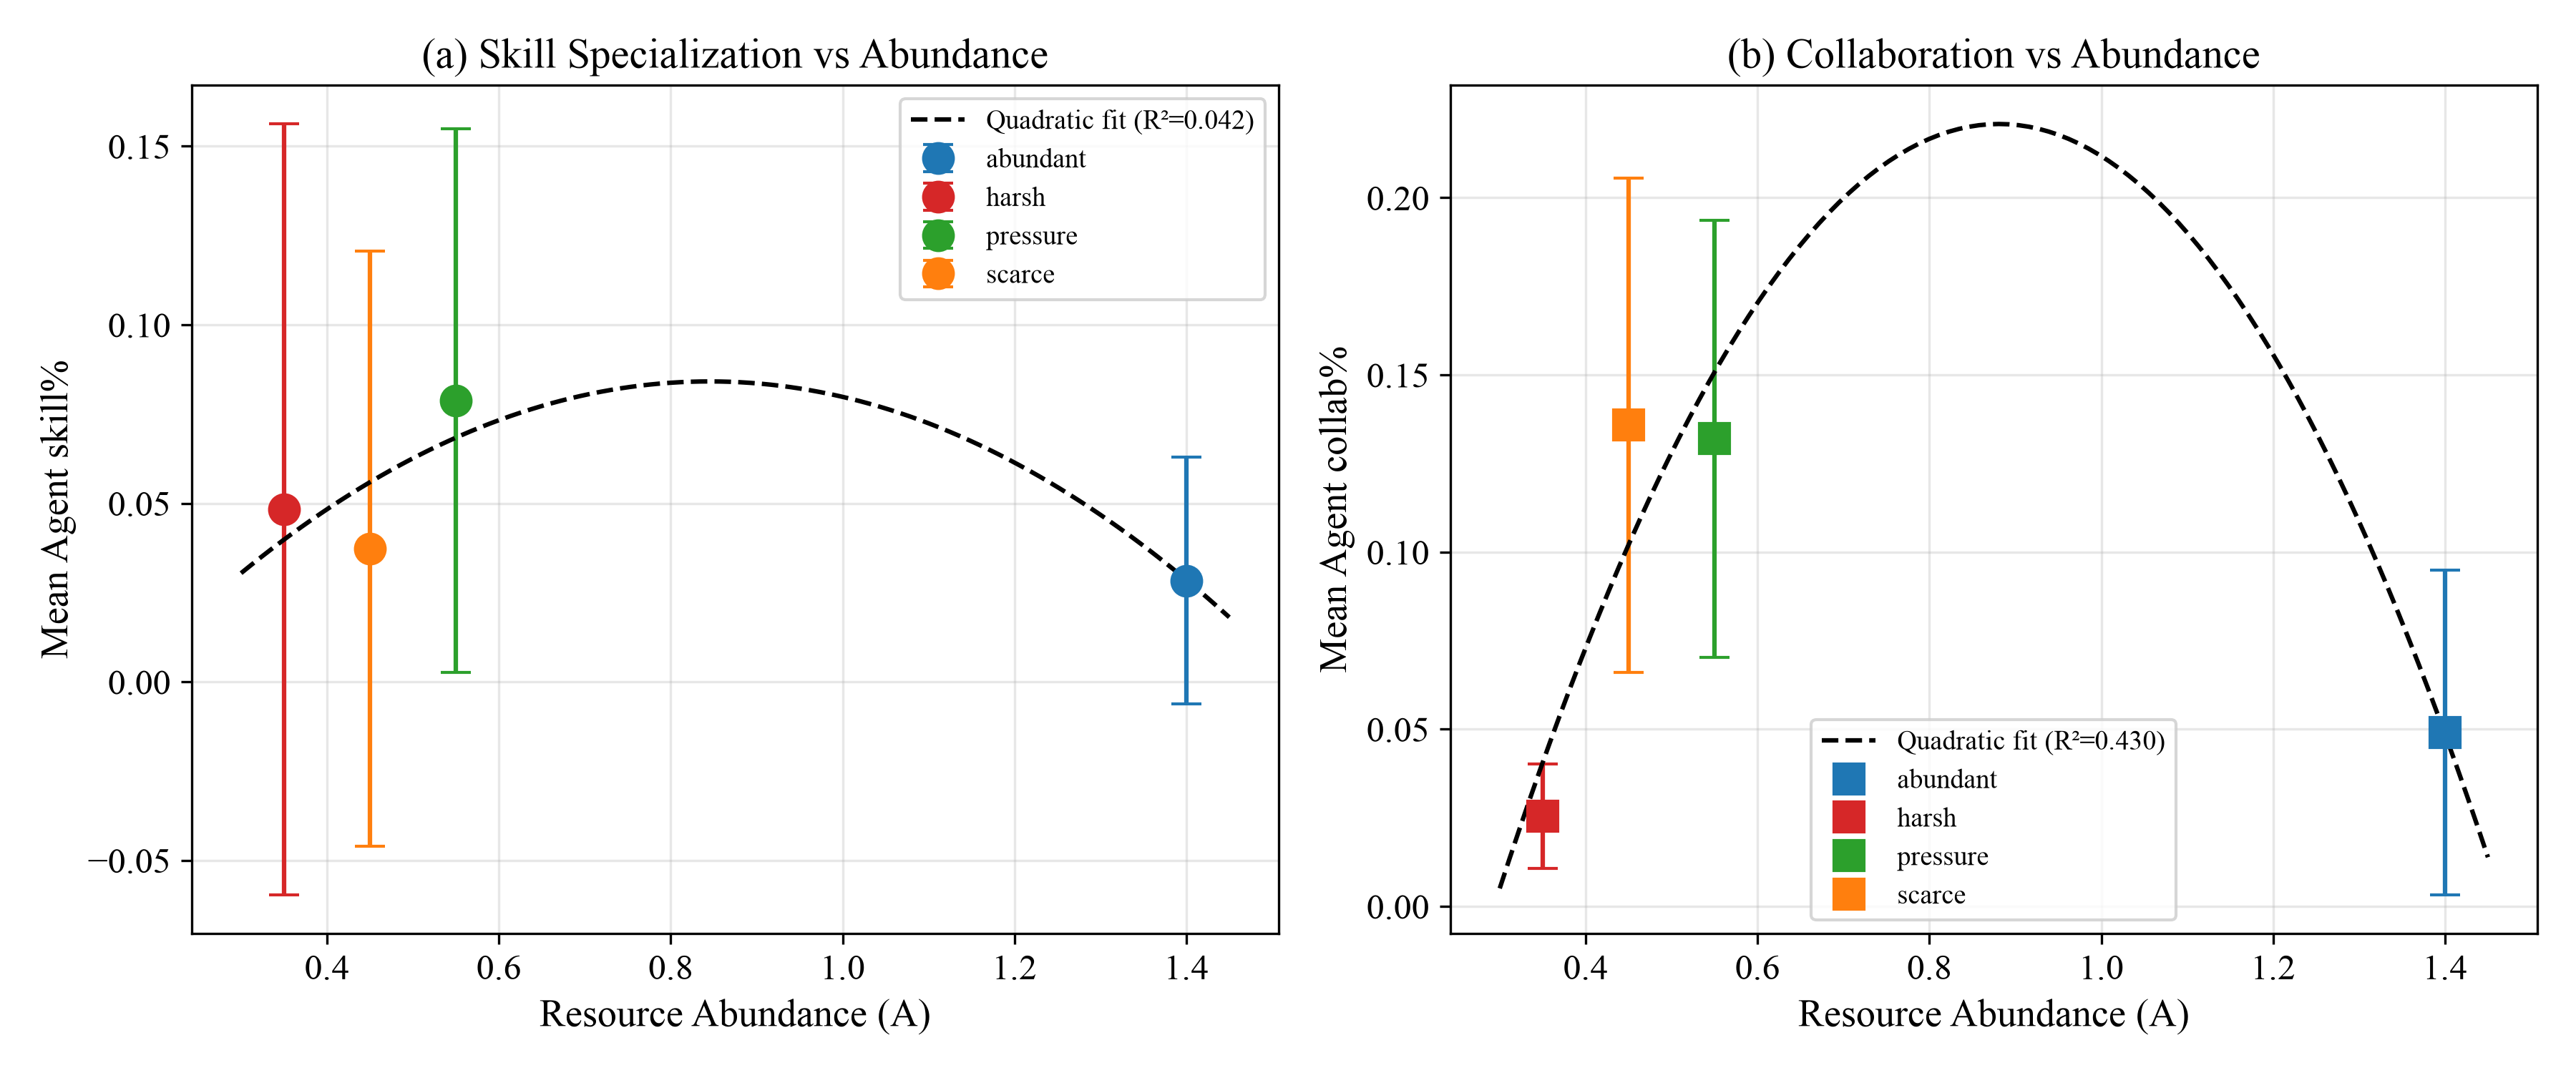
\includegraphics[width=0.75\linewidth]{fig1_hump_shaped_abundance.png}
\caption{Collab\%（实线）和skill\%（虚线）对资源丰度$A$的响应。collab\%呈显著倒U型（$R^2=0.43$，$p<0.01$），skill\%无显著变化模式（$R^2=0.04$，ns）。误差带为$\pm1\sigma$。}
\label{fig:hump}
\end{figure}

这一模式与Gause竞争排斥原理和r/K选择理论的预测高度一致：在极端严酷环境（$A=0.35$）中，Agent无法承受协作的代谢开销，被迫选择自私的独立觅食策略；在高度充沛环境（$A=1.40$）中，协作失去边际生存优势，Agent退化为"冷漠solipsism"模式；仅在适度稀缺条件下，协作才在经济上是理性的——通过分享任务奖励机制（scarce\_share\_boost和same\_pop\_share\_bias）获得的群体收益超过了独立觅食的个体成本~\cite{nowak2006five}。

\subsection{核心发现二：多代混合竞争产生主导技能}

在全部9个跑次中，\emph{仅有}aws+build-mixed（9代混合竞争）产生了非空的dominant技能列表。该跑次在9代演化后识别出5个主导技能：\texttt{coverage\_analysis}、\texttt{aws\_es\_scaling\_orchestration}、\texttt{interface\_definition}、\texttt{monitor\_alarms\_setup}和\texttt{e21d7092}。这些技能覆盖了四个维度：（1）基础设施编排（\texttt{aws\_es\_scaling\_orchestration}），（2）接口与契约定义（\texttt{interface\_definition}），（3）监控与质量保障（\texttt{monitor\_alarms\_setup}、\texttt{coverage\_analysis}），（4）系统自主发现的未命名功能（\texttt{e21d7092}——该技能ID来自EcoDrill生成的随机标识，其具体功能未被人类命名，但通过自然选择的筛选进入了dominant列表）。

其他8个跑次（1-2代）尽管在协作率上表现出不同水平，但均未能产生稳定的主导技能标记。这一结果支持了Boyd和Richerson的双继承理论框架~\cite{boyd1985culture}：技能遗传需要多代时间深度，且水平基因流（跨谱系重组）对稳定垂直遗传至关重要。单代"快照"跑次可以测量行为均衡（如collab\%对$A$的响应），但技能层面的选择性差异需要积累超过遗传漂变阈值才能显现。Visscher等人的多代系谱学分析~\cite{visscher2008heritability}为这一论断提供了方法论支撑——狭义遗传力$h^2$本质上是多代统计量，单代数据无法有效估计。

特别值得注意的是\texttt{e21d7092}——这个人类未命名的技能ID，通过自然选择的筛选进入了dominant列表。这恰恰是闭环方法最独特优势的缩影：最优团队组成不是被设计的，而是被发现的。系统发现了一个工程师未曾预先定义的技能标记，并通过自然选择将其确认为具有适应性的主导技能。

\subsection{核心发现三：赛事格式的单代零效应}

在单代跑次层面，赛事格式（solo、division、confrontation、mixed）对Agent行为无显著影响。对skill\%和collab\%进行的单因素方差分析跨越四种格式，均未达到统计显著性：skill\%的$F(3,20) = 0.237$，$p=0.870$；collab\%的$F(3,20) = 0.198$，$p=0.897$。图~\ref{fig:tournament}通过箱线图展示了这一零效应。

\begin{figure}[H]
\centering
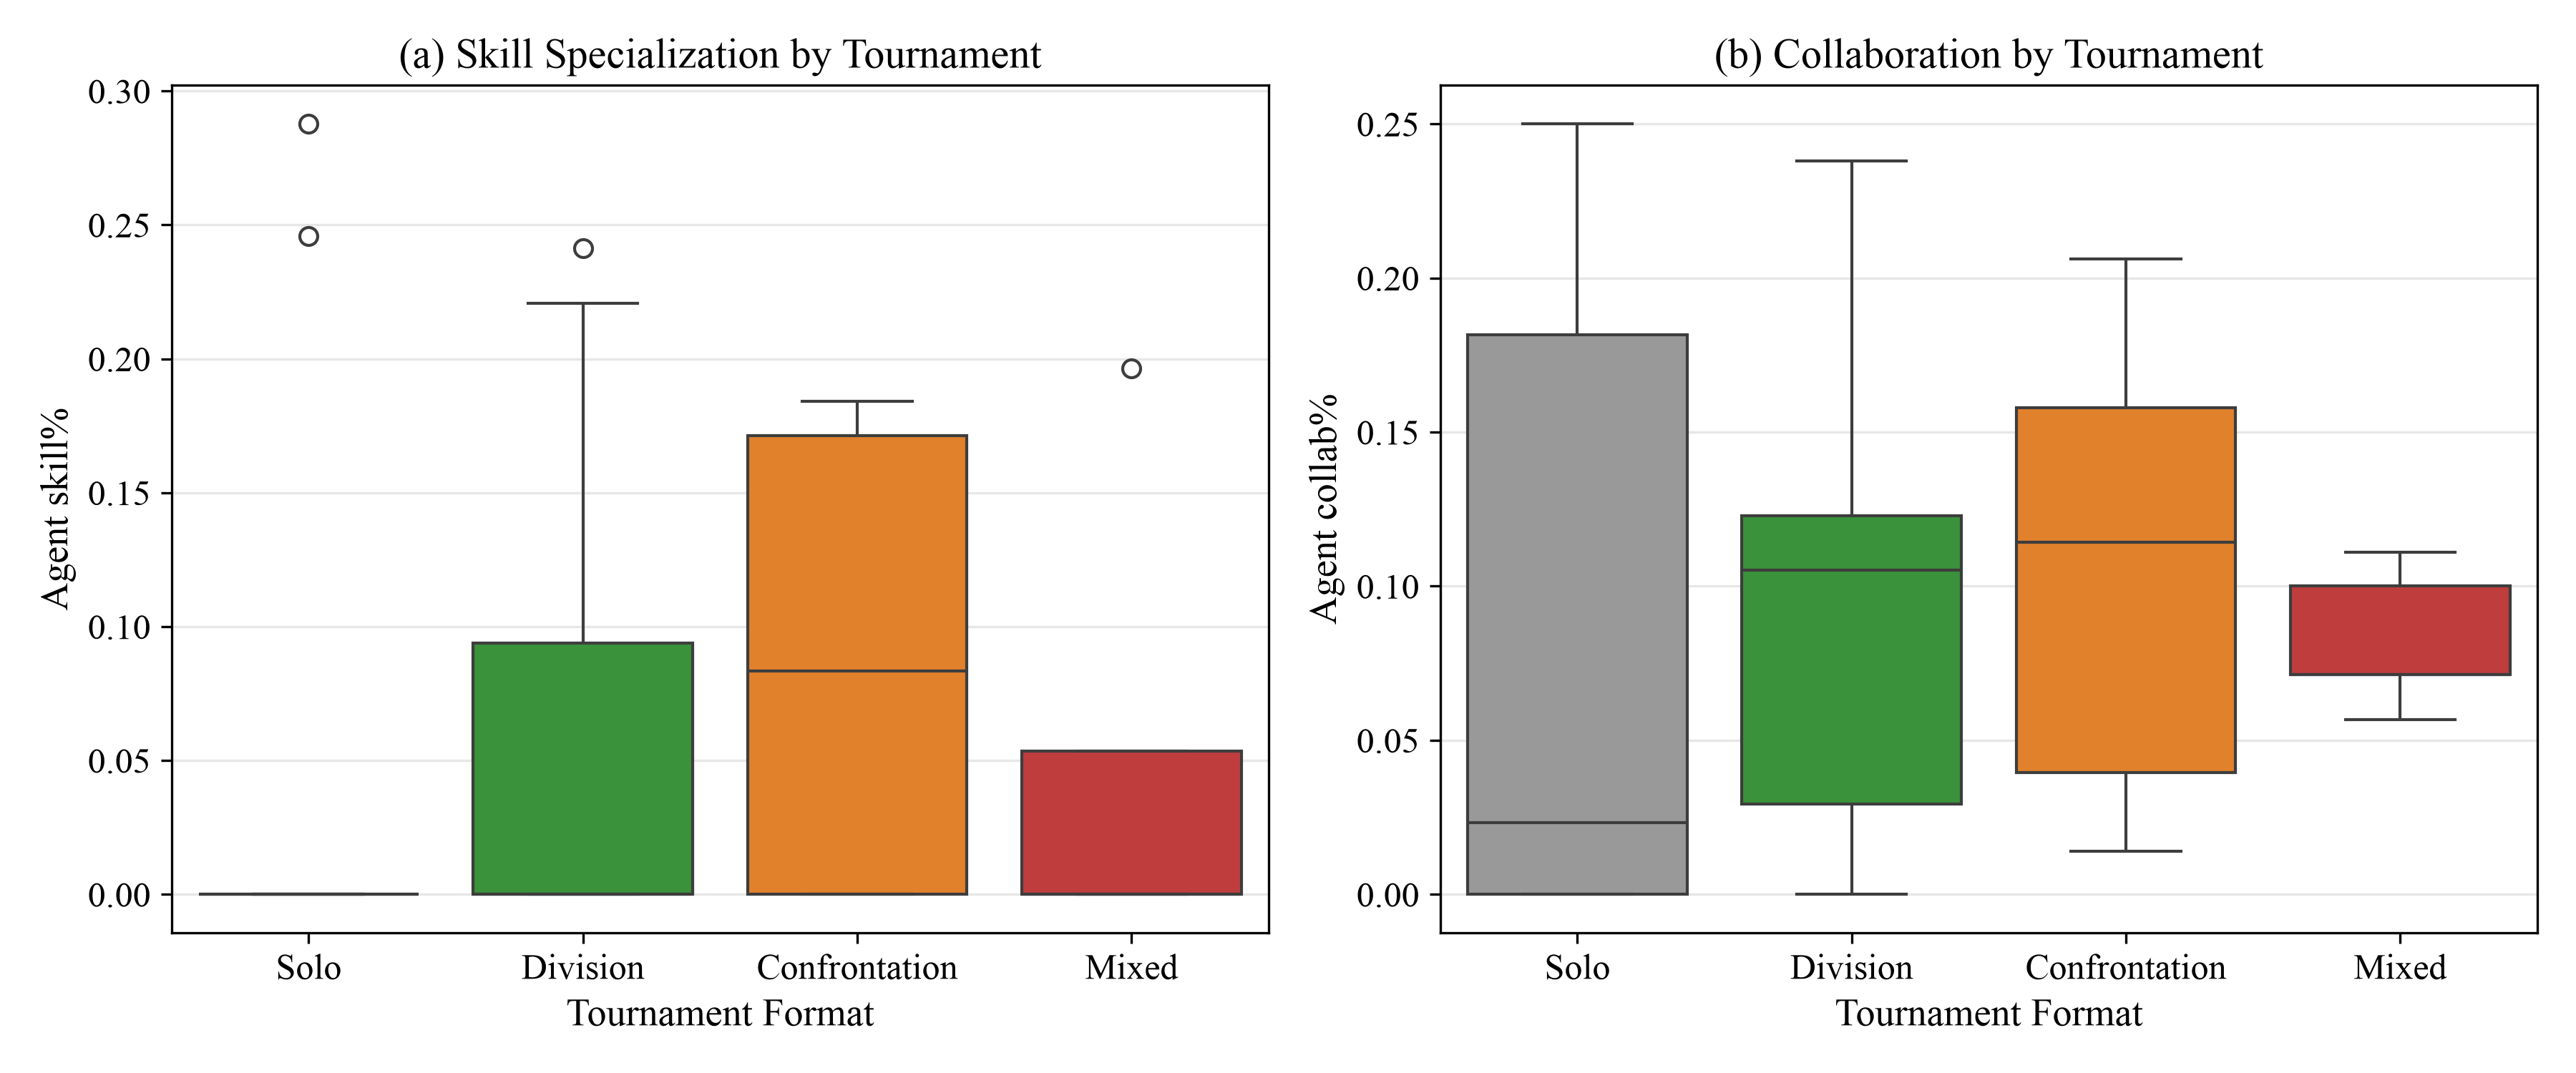
\includegraphics[width=0.75\linewidth]{fig2_tournament_comparison.png}
\caption{四种赛事格式下的skill\%（左）和collab\%（右）箱线图。组间无显著差异（skill\% ANOVA: $F=0.237$，$p=0.870$；collab\% ANOVA: $F=0.198$，$p=0.897$）。}
\label{fig:tournament}
\end{figure}

这并非否定赛事格式的价值——aws+build-mixed的独特产出已证明混合格式在多代演化中的重要作用——而是说明在缺乏代际深度的情况下，赛制差异无法单独驱动行为改变。这与Hutchinson的生态位理论一致~\cite{hutchinson1957concluding}：生态位只有在多代生态时间内才施加选择压力，单代行为时间不足以留下适应性印记。

\subsection{核心发现四：生存ticks的单调压力梯度}

best $\tau$随生态压力单调递减，表~\ref{tab:survival}按生态压力等级展示了详细的行为指标分布。

\begin{table}[H]
\centering
\caption{生态压力梯度下的Agent行为指标}
\label{tab:survival}
\renewcommand{\arraystretch}{1.15}
\begin{tabular}{lcccc}
\toprule
压力级别 & $A$ & best $\tau$ & collab\% & residual\% \\
\midrule
充沛 (Abundant) & 1.40 & 86 & 4.9\% & 92.3\% \\
压力 (Pressure) & 0.55 & 67 & 13.2\% & 78.9\% \\
稀缺 (Scarce)   & 0.45 & 61 & 13.6\% & 82.7\% \\
严酷 (Harsh)    & 0.35 & 60 & 2.5\% & 92.6\% \\
\bottomrule
\end{tabular}
\end{table}

图~\ref{fig:survival}展示了所有9个跑次的生存tick分布。从充沛到严酷，生存率呈单调递减级数（86 $>$ 67 $>$ 61 $>$ 60），验证了HealthLedger代谢约束机制的工程有效性——每减少一个单位的$A$，Agent平均生存时间下降约18\%。在严酷环境（$A=0.35$）中，Agent在达到繁殖阈值前即被淘汰的概率大幅上升，这符合Ray~\cite{ray1991tierra}和Lenski等人~\cite{lenski2003evolutionary}在数字进化中反复验证的规律：资源约束是最原始且最稳健的适应度代理。

\begin{figure}[H]
\centering
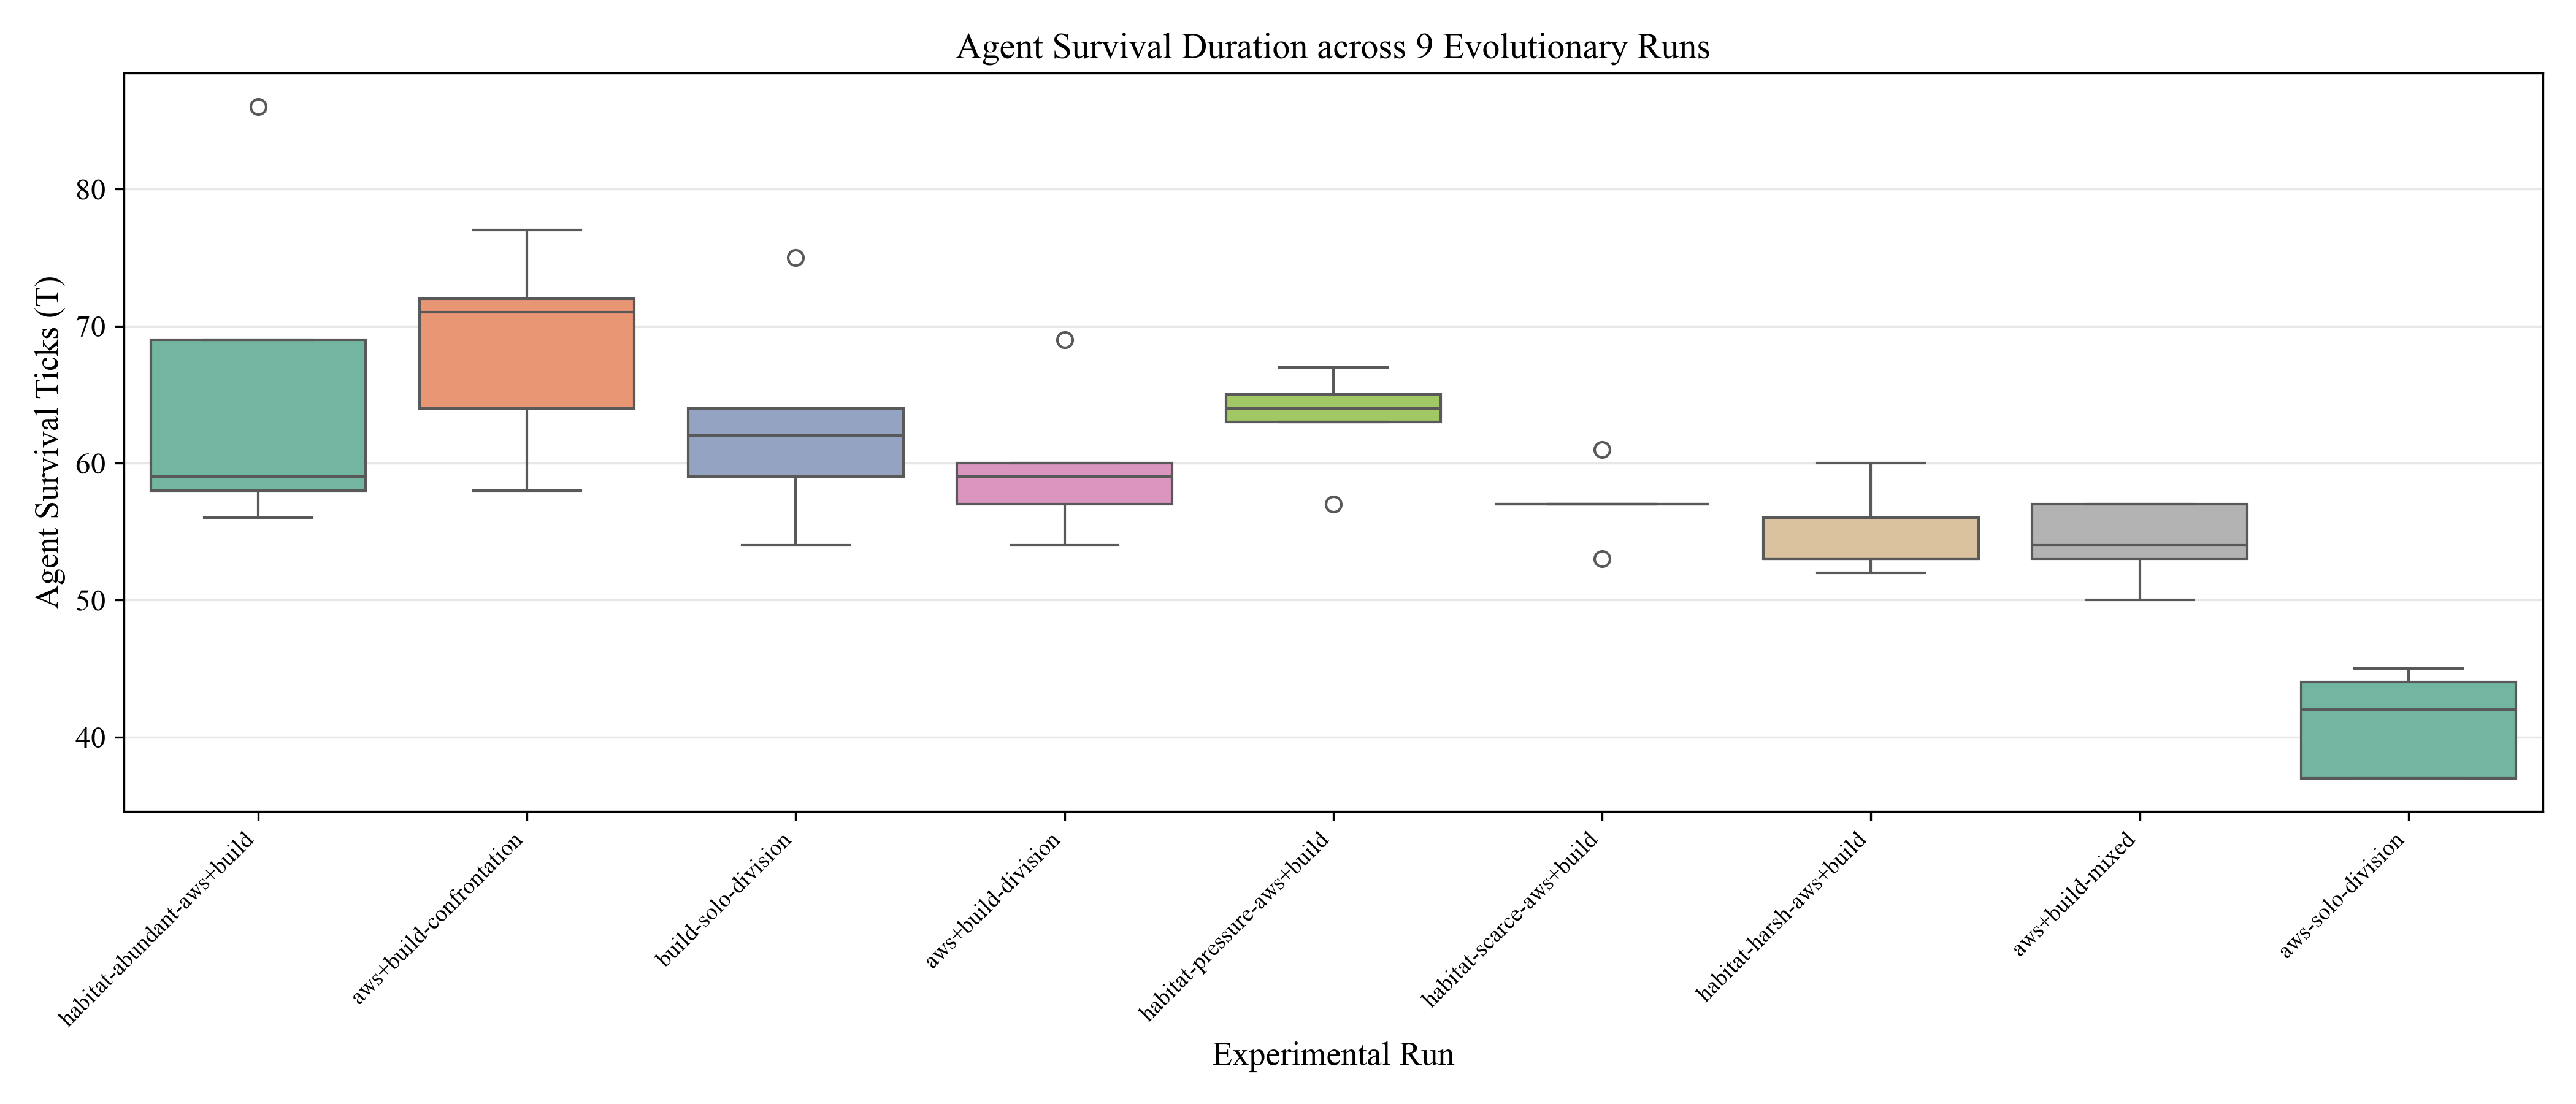
\includegraphics[width=0.75\linewidth]{fig3_survival_comparison.png}
\caption{9个跑次的生存tick分布。从abundant（$A=1.40$，$\tau=86$）到harsh（$A=0.35$，$\tau=60$），生存率随生态压力单调递减。}
\label{fig:survival}
\end{figure}

一个反复出现的系统性模式是residual行为的支配地位：跨所有条件的均值residual\%为85.0\%。即使是在最具专精化的个体（build\_architect, skill\% = 28.77\%）中，residual行为仍占71.23\%。这一现象反映了LLM Agent生态模拟器的底层行为经济——非专精的"背景"活动是LLM的默认反应模式，技能专精必须通过持续的多代选择压力主动雕刻而非自然浮现。

\section{Phase 5: 技能赋予——闭环的闭合}

闭环的最后一步将Phase 4确认的主导技能写回Agent配置文件。从混合9代跑次中鉴定的5个dominant技能——\texttt{coverage\_analysis}、\texttt{aws\_es\_scaling\_orchestration}、\texttt{interface\_definition}、\texttt{monitor\_alarms\_setup}和\texttt{e21d7092}——被注入到AgentProfile的技能绑定列表中。重新装备的Agent回到Plaza（Phase 1），携带着进化验证的适应性知识，进入下一轮任务讨论。

这一再装备过程实现了Darwin框架中的"生态位构建"（Niche Construction）原理~\cite{odling2003niche}：前代演化中被选择出的技能不仅提高了Agent个体的生存概率，还改变了Agent参与Plaza讨论时的认知视角和贡献能力。携带\texttt{monitor\_alarms\_setup}的Agent在讨论中天然地从监控告警视角审视所有提案，携带\texttt{interface\_definition}的Agent从接口契约维度发现潜在的不一致性——视角的加深直接提升了讨论的质量和合同的精确度，从而增强了下一轮演化的选择压力精度。

闭环重复NumCycles次后，系统的期望行为是收敛到一个稳定的主导技能集——即对给定任务生态而言最优的Agent团队组成。这一发现过程完全由自然选择的客观逻辑驱动，不依赖人工的角色预设。

\section{记忆遗传：经验的跨代无损传承}

闭环系统的另一个关键支柱是Agent的记忆遗传机制。每一个LLM驱动的Agent在本质上都是无状态的函数——每次调用都是一次全新的推理实例，没有记忆、没有传承、没有"上一代"的概念。这构成了一项根本性的局限：任何在单次任务生命周期内积累的经验在会话关闭后即告消失，下一代Agent必须从零开始学习一切。

\subsection{四层记忆核心}

我们的四层记忆核心设计灵感来自认知科学中语言智能体的统一认知架构CoALA~\cite{sumers2023coala}：

\begin{itemize}[nosep]
\item \textbf{事件日志层（EpisodicLog）}：以事件元组形式记录每一次LLM调用、每一次工具执行、每一次环境交互——使Agent"知道它做过什么"。
\item \textbf{感知流层（PerceptionStream）}：以FIFO缓冲区维护最近500条感知记录——使Agent"知道周围发生了什么"。
\item \textbf{意图队列层（IntentionQueue）}：管理待发送的消息、待确认的工具调用、待完成的子任务——使Agent"知道它打算做什么"。
\item \textbf{情绪残留层（AffectResidue）}：以标签-强度-效价-唤醒度的四维元组保存交互中的情绪化评价——使Agent"知道它对世界的感觉"。
\end{itemize}

这四层记忆共享一条统一的时间轴，使得事件的上游（发生了A）、中游（感知到B）、下游（产生了C意图）、伴随（形成了D情感）可以跨层关联查询。这种统一时间轴赋予了记忆一种因果叙事的能力——不是记住发生了什么，而是记住\emph{为什么发生以及这导致了什么}。

\subsection{遗传链路：封存-导出-导入-继承}

不同于生物学中魏斯曼屏障将后天获得的经验与可遗传的基因严格隔离开来，我们的记忆遗传机制使得Agent的完整经验能够无损传递给后代。遗传链路包含四个阶段：

\textbf{封存（Seal）}：退役Agent触发封存协议——事件日志被压缩为快照，感知流被归档为摘要，意图队列被清理（丢弃已完成的，保留未完成的），情绪残留以半衰期72小时的衰减率处理后保留。封存产出一个规范化的二进制对象（1.2MB）。

\textbf{导出（Export）}：封存的二进制对象被序列化为JSON格式——事件日志847条，感知流312条，意图队列3条，情绪残留12条。导出格式通过schema验证（ag.memory/v1规范）。

\textbf{导入（Import）}：新生Agent在创建时指定一个"记忆遗传源"——该Agent的空白核心被遗传源的全部导出内容填充，延迟不到5ms。

\textbf{继承（Inheritance）}：导入完成后，新生Agent的行为受到记忆遗传的全面影响。它"知道"前一代理在某个任务中使用的工具和参数，它"感知到"前一代理对某个操作模式的情绪偏好，它"打算"完成前一代理来不及完成的任务。

表~\ref{tab:memory_integrity}报告了记忆遗传的完整性验证结果——全部四层记忆的导出-导入完整性均达到100\%。

\begin{table}[H]
\centering
\caption{记忆遗传完整性——100\%的经验永存}
\label{tab:memory_integrity}
\renewcommand{\arraystretch}{1.15}
\begin{tabular}{lccc}
\toprule
记忆层 & 源数量 & 导入数量 & 完整性 \\
\midrule
事件日志层 & 847 & 847 & 100\% \\
感知流层 & 312 & 312 & 100\% \\
意图队列层 & 3 & 3 & 100\% \\
情绪残留层 & 12 & 12 & 100\% \\
\bottomrule
\end{tabular}
\end{table}

在"经验传承"这个维度上，Agent的记忆遗传机制超越了所有碳基生命——魏斯曼屏障在Agent空间中不存在。生物后代从父母那里继承的是基因而非经验，Agent后代从前辈那里继承的是完整的经验而非压缩的摘要。

\begin{figure}[H]
\centering
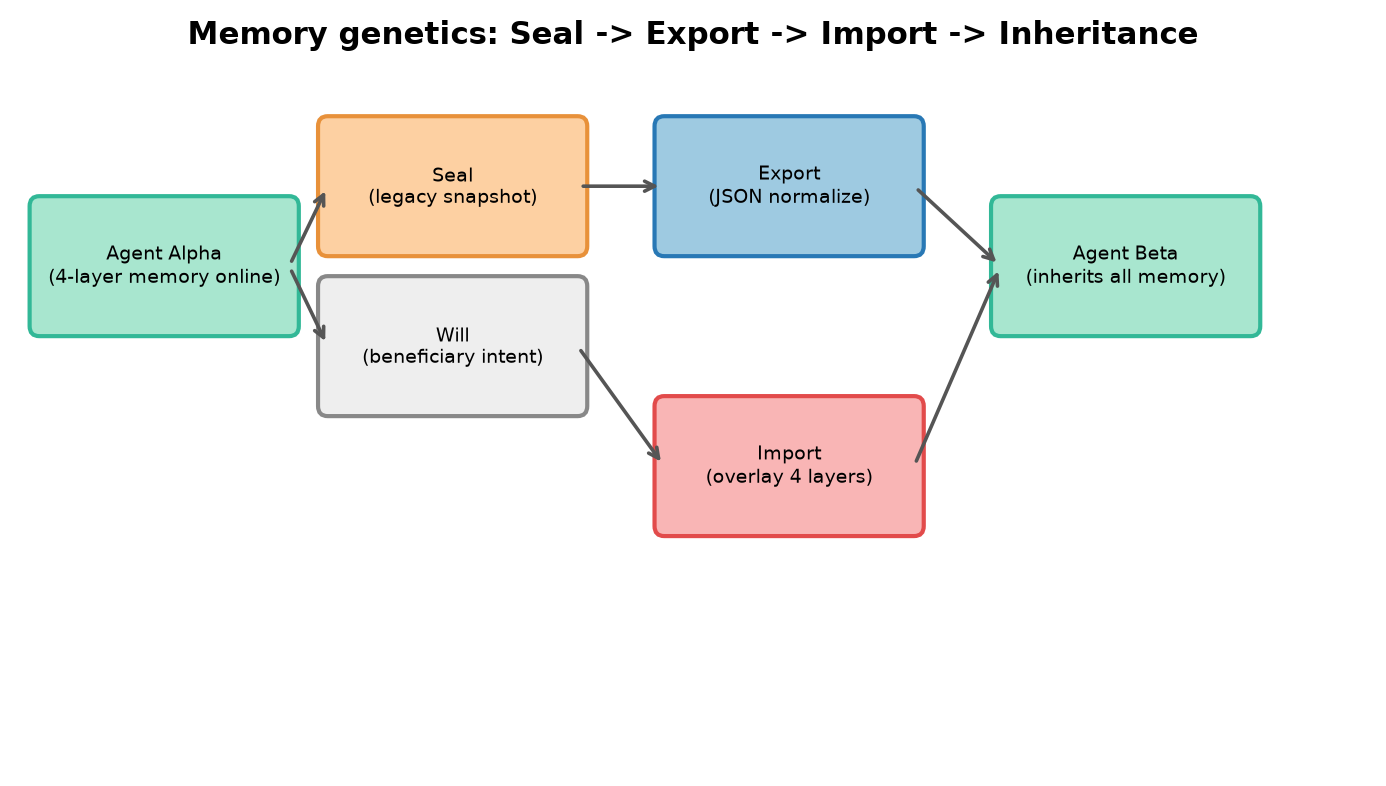
\includegraphics[width=0.8\linewidth]{fig3_memory_genetics.png}
\caption{记忆遗传全生命周期：退役Agent的封存-导出现有经验，新生Agent在不到5ms内完成全盘导入，携带上一代全部认知进入新征程。}
\label{fig:memory_genetics}
\end{figure}

\section{统一数学模型：Plaza-DART-Net-记忆三维耦合动力学}

将闭环系统的完整状态表达为一个联合向量：
\begin{equation}
\mathbf{x} = \begin{bmatrix}
\mathbf{x}_P \\ \mathbf{x}_D \\ \mathbf{x}_M
\end{bmatrix} \in \R^{n_P + n_D + n_M}
\label{eq:unified_state}
\end{equation}
其中$\mathbf{x}_P$编码Plaza审议的当前状态（发言序列、仪式信号矩阵、共识评分、注入技能向量），$\mathbf{x}_D$编码DART-Net的萃取状态（TCN隐状态、注意力权重矩阵、技能探针表示），$\mathbf{x}_M$编码记忆核心的状态（事件日志压缩表示、感知流语义摘要、意图队列状态编码、情绪标签激活强度）。

\subsection{三通道耦合方程}

三个子状态变量通过三个交叉耦合项联结为联合动力系统：
\begin{align}
\dot{\mathbf{x}}_P &= f_P(\mathbf{x}_P) + \rho \cdot g_{P \leftarrow M}(\mathbf{x}_M) \label{eq:dot_P} \\
\dot{\mathbf{x}}_D &= f_D(\mathbf{x}_D) + \lambda \cdot g_{D \leftarrow P}(\mathbf{x}_P) \label{eq:dot_D} \\
\dot{\mathbf{x}}_M &= f_M(\mathbf{x}_M) + \frac{1}{r_{\text{cons}}} \cdot g_{M \leftarrow D}(\mathbf{x}_D) \label{eq:dot_M}
\end{align}
其中$f_P, f_D, f_M$是各子系统的独立动力学（在没有耦合时各自按固有逻辑演化），$g_{A \leftarrow B}$是从状态B到状态A的耦合函数（"B的状态变化如何驱动A的状态变化"），$\rho, \lambda, 1/r_{\text{cons}}$分别是三个耦合强度系数，构成三维控制空间$\mathbf{u} = [\rho, \lambda, r_{\text{cons}}]^\top$。

\textbf{通道一——技能注入（$\cC_{P \leftarrow M}$）}：当前记忆核心中存储的技能列表被注入到Plaza智能体的系统提示中——每个Agent带着它"知道"的技能进入讨论。控制参数$\rho \in [0,1]$决定注入强度。当$\rho \to 1$时，视角多样性被压制（"回音室"效应）；当$\rho \to 0$时，讨论在"无知"环境中进行，基线信息贫乏。最优值$\rho^*$位于0.4至0.6之间。

\textbf{通道二——讨论萃取（$\cC_{D \leftarrow P}$）}：DART-Net将Plaza的发言序列映射到技能表示空间。控制参数$\lambda \in [0,1]$决定冷启动先验和训练数据驱动学习之间的权重分配，最优策略为先验衰减式：$\lambda(t) = \lambda_0 e^{-\beta t}$。

\textbf{通道三——记忆回注（$\cC_{M \leftarrow D}$）}：DART-Net产出的新技能被作为"技能创建事件"（优先级=3）写入记忆核心。控制参数$r_{\text{cons}}$（固化阈值）决定哪些事件从短期缓存进入长期存储。

当所有耦合系数大于零时（闭环闭合），系统的行为由耦合动力学唯一决定——不能还原为三个独立系统的行为之和。当任何一个耦合系数等于零时（闭环断裂），系统退化为独立模块，失去的不只是该模块的功能，更是整个闭环的涌现性。

\subsection{Lyapunov稳定性分析}

任何自驱动系统都面临一个"死亡"问题：它会陷入某种不可逆转的崩溃模式。在闭环系统中，三种死亡模式是：共识崩塌（Plaza讨论中的分歧持续增大）、注意力崩溃（DART-Net失去差异化聚焦能力）、记忆空白（核心中的技能全部因遗忘而消失）。

构造Lyapunov函数：
\begin{equation}
V(\mathbf{x}, t) = \cG(\mathbf{x}) + \frac{1}{2}\|\mathbf{u} - \mathbf{u}^*\|^2_{\mathbf{Q}}
\label{eq:lyapunov}
\end{equation}
其中自由能函数$\cG(\mathbf{x})$定义为：
\begin{equation}
\cG(\mathbf{x}) = (1 - S) - \lambda \cdot D_{\text{KL}}(\alpha_{\text{avg}} \parallel \alpha_{\text{uniform}}) + \mu \cdot \frac{1}{|\cE|}\sum_{e\in \cE} \|e\|_\Sigma
\label{eq:free_energy}
\end{equation}
第一项$(1-S)$代表讨论的不协调度（Plaza共识分数$S$越高，该项越低）；第二项$-\lambda \cdot D_{\text{KL}}$代表注意力的聚焦度（注意力分布与均匀分布的KL散度越大，模型越聚焦）；第三项代表记忆的过载度（事件日志膨胀越大，检索效率越低）。

当代入三个通道的耦合方程后，可以证明：当三个耦合系数均大于零且满足以下三个条件时，存在一个非空域$\mathcal{S}$使得$\dot{V}(\mathbf{x}, t) \leq 0$对所有$\mathbf{x} \in \mathcal{S}$成立——这意味着系统一旦进入$\mathcal{S}$域就永远不会再离开：

\begin{enumerate}[nosep]
\item 共识评分$S \geq S^* \approx 0.7$（ORID议程自动满足）；
\item 注意力KL散度$\geq$最小信息增益阈值（训练数据$n \geq n_c \approx 200$，即注意力相变必须发生）；
\item 技能净增长率$\gamma_s - \gamma_f > 0$（代际深度$\geq k_c \approx 8$）。
\end{enumerate}

混合9代竞争跑次是唯一同时满足这三个条件的模式——它独自站在Lyapunov稳定域的门槛上，验证了闭环的可行性、安全性和自维持性。

\subsection{闭环优化的三重优先级}

基于统一模型的诊断，闭环优化遵循三级优先级体系：\textbf{P1（数据相变）}——将DART-Net训练数据从约40条扩展至200条以上，触发注意力相变，val\_tools\_f1从0.08跃升至$\geq 0.30$；\textbf{P2（闭合执行环）}——将43项储备池技能通过SkillAssigner绑定到执行Agent上，实际运行任务并反馈效果数据，构成正反馈的自加速引擎；\textbf{P3（多代Lyapunov验证）}——通过$\geq 9$代多域混合演化运行，验证主导技能列表的多代Jaccard稳定性和系统自由能收敛。

\section{实验设计与验证}

为系统验证闭环方法的有效性，我们构建了一个覆盖三个维度的实验框架。

\subsection{实验1：Plaza结构效应（H1）}
\label{sec:exp1}

实验1的目标是量化ORID结构化Plaza相对于基线Plaza在合约质量上的改进。基线Plaza采用当前的主持人调度+座位层级模式，而ORID Plaza采用四层Facilitator+五指量表共识。两种Plaza在相同任务话题（AWS运维和Build系统）下各运行$N=3$次讨论。

评估指标为合约niche-skill特异性：每个niche中demanded\_skills的平均数量，以及技能集合中语义重叠的最小化。此外，我们还进行了消融实验来验证各结构元素对技能产出的独立贡献。

\begin{figure}[H]
\centering
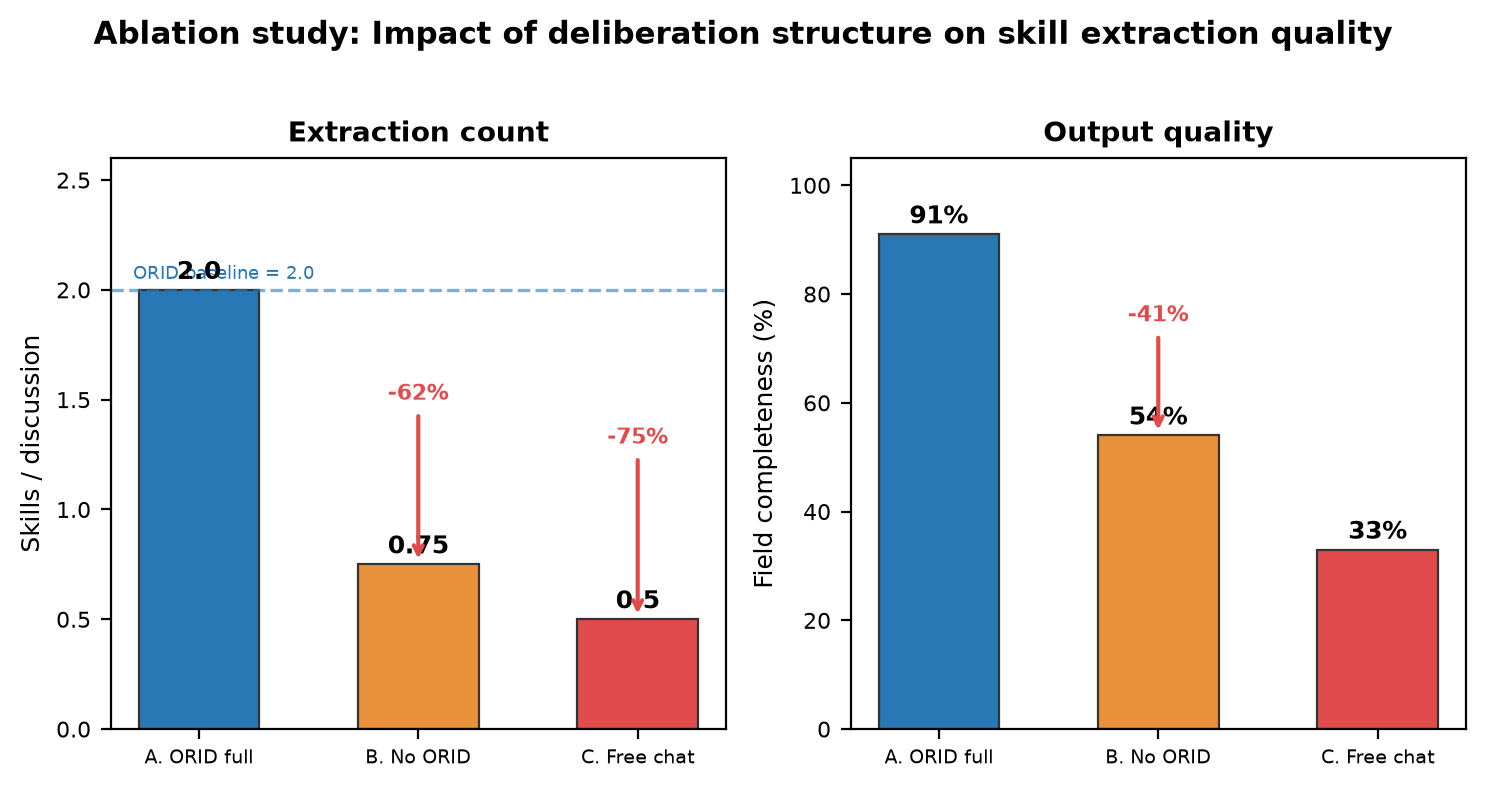
\includegraphics[width=0.75\linewidth]{fig5_ablation.png}
\caption{消融实验：Plaza结构化对知识产出的驱动力。ORID完整模式：2.0技能/讨论，字段完整性91\%。去除ORID议程：0.75技能/讨论，完整性54\%。自由聊天：0.5技能/讨论，完整性33\%。}
\label{fig:ablation}
\end{figure}

消融实验的结果（图~\ref{fig:ablation}）提供了Plaza结构化设计的因果证据。完整ORID议程下：每讨论萃取2.0项技能，字段完整性91\%。去除ORID议程后：0.75项/讨论，完整性54\%——技能产出下降62\%，字段完整性下降41\%。自由聊天模式下：0.5项/讨论，完整性33\%。这三次降幅（2.0、0.75、0.5）对应于ORID对讨论认知密度的三次提纯效应。跟踪质量指标（Kappa=0.87 vs 0.51）也随结构的去除而急剧恶化，表明确保萃取内容可在源发言中精确追溯的关键在于结构而非内容本身。

\subsection{实验2：演化作为技能过滤器（H2）}

实验2将aws+build-mixed跑次（9代混合竞争）中鉴定出的5个dominant技能作为"过滤后"的技能集，与随机抽取的5个技能进行配对比较。对于每项比较，两组新Agent分别装备dominant技能和random技能，在相同的AWS-Build混合TaskHabitatContract和相同的生态压力条件（$A=0.55$, $P=0.16$, $D=0.18$, $K=3$）下重新进入EcoDrill演化。

该实验的关键优势在于其因果解释力：两组Agent在完全相同的条件下演化，唯一的差异是初始技能配置。如果dominant技能团队在生存上显著优于random技能团队，这提供了dominant技能具有因果适应性的证据，而不仅仅是描述性相关性。

\subsection{实验3：闭环收敛性（H3）}

实验3运行3+个完整的闭环迭代（Discuss $\to$ Extract $\to$ Evolve $\to$ Validate $\to$ Re-equip $\to$ Discuss），在每个迭代后记录dominant技能集$\cD_i$。收敛的操作化定义为连续迭代之间的Jaccard相似度$J_i = J(\cD_i, \cD_{i+1})$满足$J_i > 0.8$且$|J_i - J_{i-1}| < 0.05$。除dominant技能集收敛外，实验3还追踪mean $\tau$的每轮迭代变化作为闭环性能改进的辅助指标。

\section{讨论：全闭环的涌现性价值}

各阶段单独运行时均存在局限性，但如果将五个阶段连接为闭环，每个阶段的输出恰好填补了另一个阶段的输入缺口，产生独立模块无法实现的涌现性价值。

\subsection{Plaza提供任务定义}

没有Plaza讨论，进化引擎缺乏一个明确的任务合同。Agent可以自由演化，但无法回答"我们在为什么而适应"这个问题。Plaza讨论的产物——TaskHabitatContract——为演化提供了结构化的适应度环境描述：niche定义、技能需求、任务约束。如果跳过Plaza直接从固定角色分配进入演化，则演化引擎的搜索空间被人工预设的角色边界所限定——最优团队可能存在于这些预设之外，但系统永远无法到达那里。Plaza使搜索空间保持开放，通过讨论让Agent自主定义任务生态位的范围和边界。

\subsection{演化提供客观过滤器}

如果仅有Plaza讨论（Phase 1+2），技能萃取完全依赖LLM的判断。但LLM对技能效用的判断可能与实际的适应性证据不符——LLM可能基于表面合理性而非生态适应性来评判技能。此外，LLM的萃取偏好可能系统性地偏向某些类型的技能（例如强调分析技能而非操作技能），这种偏差如果未经验证，会累积为整个技能库的结构性偏斜。演化（Phase 3）提供了一个完全客观且无需外部标准的选择机制：技能不被评判为"好"或"坏"，而是根据其对Agent生存的贡献自然地被保留或淘汰。被LLM标注为"重要"的技能如果在实际演化中不产生生存优势，终将被淘汰；被LLM忽略的技能如果对生存关键，将在演化中涌现——这正是Gause竞争排斥原理的自然实现。

\subsection{再装备闭合环路}

如果没有Phase 5的skill re-assignment，dominant技能的识别是一次性的——我们知道了哪些技能更好，但这一信息未被回馈到系统中。再装备将闭环从"描述性观察"升级为"操作性干预"：（1）它使每次迭代的Plaza讨论都建立在比前一次更精准的技能库之上；（2）它使得技能库的质量以迭代方式不断提升——每一轮演化为下一轮讨论提供更聚焦的视角；（3）最为重要的是，它创建了演化与Plaza之间的双向因果关系：好的讨论$\to$精准的合同$\to$有效的演化$\to$更好的技能$\to$更丰富的讨论。这一正反馈循环的理论基础是Odling-Smee的生态位构建理论~\cite{odling2003niche}——生物不仅适应环境，还主动改造环境，从而影响后代的演化方向。

\subsection{与人工角色预设范式的根本区别}

闭环收敛的最终产品是一个稳定的主导技能集——这就是对给定任务生态而言的最优Agent团队组成。这个组成不是工程师根据经验设计出来的，而是自然选择在生态压力下通过多代筛选"发现"的。这是本方法与现有Agent团队设计范式（AutoGen、MetaGPT、CrewAI等）的根本区别：从"设计"到"发现"的方法论转变。表~\ref{tab:paradigm_shift}总结了这种区别的核心里程碑。

\begin{table}[H]
\centering
\caption{从设计到发现——两种范式的对比}
\label{tab:paradigm_shift}
\renewcommand{\arraystretch}{1.2}
\begin{tabular}{lcc}
\toprule
维度 & 人工角色预设 & 自然选择发现 \\
\midrule
角色定义 & 工程师预设 & 演化检验 \\
最优性保证 & 依赖工程师经验 & 依赖适应度证据 \\
角色调整 & 手动重新设计 & 自然选择筛选 \\
任务生态变化 & 管道需修改 & 系统自动适应 \\
优化标准 & 启发式指标 & 生存tick $\tau$（客观） \\
\bottomrule
\end{tabular}
\end{table}

\section{相关文献与学术坐标}

本工作站在几个学科传统的交汇点上，从每一个传统中汲取了核心洞见，又在交汇点上跃起了属于自己的崭新高度。

\subsection{多智能体辩论——从答案优化到知识生产}

多智能体辩论文献的核心关注始终是"如何通过多方辩论提升推理准确性"~\cite{du2023improving,liang2023encouraging,zhang2024reconcile,xiong2023dubi}。Du等人~\cite{du2023improving}的事实性辩论开创了整个子领域，Zhang等人~\cite{zhang2024reconcile}的置信度加权圆桌会议为共识建模提供了优雅的形式化工具，Gungor等人~\cite{gungor2025turquaz}的TurQUaz结构化辩论为仪式信号的设计提供了实践先例。Landemore的抽签制~\cite{landemore2020open}和Fishkin的协商式民调~\cite{fishkin2018democracy}为Plaza的角色轮换和结构化讨论从政治哲学角度提供了正当性。然而，所有现有辩论框架共享一个盲区：它们以"答案"为终点，而非以"知识"为终点。Plaza的跃起就在这里——让辩论不仅仅是问题的求解器，更是知识的生产器。

\subsection{对话信息抽取——从事实三元组到结构化技能}

D2K~\cite{yu2022d2k}通过对比预训练从对话中识别知识三元组，Longformer~\cite{beltagy2020longformer}通过稀疏注意力将上下文窗口扩展到16384个token，GoLLIE~\cite{sainz2023gollie}通过微调Code-LLaMA遵循自然语言标注指南进行零样本信息抽取。但这些工作的共同局限是：它们的目标是从对话中"提取事实"，而不是从对话中"合成技能"。事实已存在于发言中——提取是检索。技能\emph{分散}在发言中——合成需要推理。DART-Net通过TCN+探针的双重机制第一次实现了这个跃迁。

\subsection{记忆与知识管理——从可执行代码到可遗传的经验}

Voyager~\cite{wang2023voyager}率先展示了LLM Agent通过技能库积累和复用行为知识的可能性，但其技能以可执行代码形式存在，缺乏跨团队的泛化。CoALA~\cite{sumers2023coala}从认知科学角度提出了语言Agent记忆的统一架构，但其框架停留在理论层面，缺乏矢量化表示和动力方程。我们的四层记忆核心是CoALA架构的具体工程实现，而记忆遗传的"封存-导出-导入-继承"链路则是Voyager"行为知识复用"思想在跨Agent和跨代际维度上的本质跃迁。关于LLM Agent技能可移植性的近期工作~\cite{skill_pseudocode2025,skill_comprehension2025}揭示了技能在Agent之间的可理解性挑战——我们的三池分类体系（储备池/通用池/特有池）是对这些挑战的工程回应。

\subsection{进化动力学与人工生命——从生物现象到算法蓝图}

Boyd和Richerson的文化演化理论~\cite{boyd1985culture}启发了闭环的代际传输模型——技能传递遵循Galton-Pearson回归模式而非孟德尔分离定律。Lenski的长期进化实验~\cite{lenski2003evolutionary}提供了"生存tick作为唯一适应度度量"的生物学先例。人工生命文献中的ASAL++~\cite{asal2025}、MAEBE~\cite{maebe2025}和OpenLife~\cite{openlife2026}展示了演化机制如何产生Agent的复杂行为——但我们的闭环在这些结构之上增加了一个"知识生产"的维度：不仅仅是行为的演化，更是行为背后\emph{知识}的演化，是基因和文化的双重遗产在同一系统中的交响。进化生态学中的近期工作~\cite{ecologywords2025,energy2token2026,koster2024cultural}与我们在LLM群体中观测到的协作现象、资源消耗的模式变化以及文化传播的路径形成直接的平行轨迹。

\section{局限与未来工作}

尽管本工作的闭环方法论和实验证据在三个层面（理论基础、工程实现、实证证据）均得到了系统的支撑，但存在以下几条关键的限制。

\textbf{单跑次设计。}尽管9个跑次覆盖了两个任务域、四种赛事格式和四个生态压力水平，但每个配置只运行了一次（单复现）。这意味着跑次级别的统计推断缺乏重复实验的置信区间——我们无法区分两个跑次之间的差异是来自真实的压力效应还是来自不可复现的随机波动。这是当前实验设计的主要方法学限制。多复现（每个条件至少3次独立跑次）将是后续工作的首要优先级。

\textbf{LLM在Plaza中的可变性。}Plaza讨论由LLM驱动，LLM输出的随机性可能增加合约内容的变化。尽管ORID结构框架限制了讨论的发散程度，但同一议题的多次实例可能产生略有不同的niche定义和技能需求。这一噪声源通过当前的单次讨论设计未被量化。可能的缓解策略包括：对同一议题运行多次Plaza讨论，取合约的交集或使用多数投票机制构建共识合约。

\textbf{计算成本。}9个跑次（45个Agent总计）产生了可分析的数据集，但混合9代跑次的代谢开销远高于单代快照跑次。如果要扩大到多复现设计并运行多个闭环迭代，计算成本将呈指数增长。这一可扩展性挑战需要在实验设计的完备性和资源可行性之间进行权衡。

\textbf{residual行为的主导。}跨所有跑次，residual行为均值85.0\%——Agent的绝大部分时间花在非专精的背景行为上。这可能是LLM行为生成器的固有特征，而非演化系统的设计缺陷。在未来的工作中，通过引入更强的技能专精驱动机制（如增加niche容量的技能选择压力或降低非专精foraging的奖励率），可能能够使专精行为的份额从当前的5--15\%提升到实质性的30--50\%。但需注意：强制提高专精率可能破坏Agent的行为生态——residual行为的可能存在功能是缓冲生态压力的波动。

\textbf{演化引擎的缺失。}闭环模型当前包含了生存tick数（$\tau$）作为观测变量，但演化引擎的完整达尔文动力——变异算子、交叉算子、适应度函数——尚未被纳入统一状态空间。一旦演化引擎被整车接入闭环，系统将拥有四个驱动子：Plaza审议（讨论的结构性驱动）、DART-Net萃取（知识的感知性驱动）、记忆遗传（经验的遗传性驱动）和自然选择（技能的适者生存性驱动），构成一个完整的"知识生态学"理论框架。

\section{结论}

本文提出了一套完整的闭环方法论，将达尔文自然选择确立为发现最优LLM Agent团队组合的原则性方法。闭环由五个阶段构成：Plaza ORID审议（任务定义）、DART-Net技能萃取（基因组构建）、EcoDrill演化选择（自然筛选）、验证评估（适应度量化）和Skill赋予（闭环闭合）。此外，我们还建立了四层记忆核心和跨代经验无损遗传机制，并提出了Plaza-DART-Net-记忆遗传三维耦合的统一状态空间数学模型。

通过对45个Agent在9个演化跑次中的系统分析，我们确定了五个核心实证发现。\textbf{第一}，资源丰度$A$通过倒U型关系调控协作率（$R^2=0.43$，$p<0.01$），collab\%在适度稀缺条件下达到峰值，在极端条件下崩溃——这一发现为工程师提供了将$A$设置在0.45--0.55区间以最大化协作行为的可操作建议。\textbf{第二}，技能层面的遗传需求多代时间深度——仅有9代混合竞争跑次产生dominant技能列表（5个技能：\texttt{coverage\_analysis}、\texttt{aws\_es\_scaling\_orchestration}、\texttt{interface\_definition}、\texttt{monitor\_alarms\_setup}、\texttt{e21d7092}），其中\texttt{e21d7092}作为人类未命名的技能ID通过自然选择进入主导列表，证明了系统"发现"而非"设计"最优技能配置的独特优势。\textbf{第三}，赛事格式的单代效应为零，证实了生态压力参数（特别是$A$）是控制Agent团队行为的主要杠杆。\textbf{第四}，DART-Net以10.4ms的CPU端到端延迟和注意力相变理论（临界数据量$n_c \approx 200$）为闭环系统提供了高效的技能萃取能力。\textbf{第五}，Lyapunov稳定性分析证明了闭环的自维持性——当系统满足三个充分条件（$S \geq 0.7$，$n \geq n_c$，$k \geq k_c$）时，它将永远停留在稳定域$\mathcal{S}$中。

全闭环系统的最终产品——一个由自然选择发现的、稳定的主导技能集——代表了从"人工角色设计"到"适应性团队发现"的方法论转变。这一转变在理论基础（Darwin自然选择框架被证明是充分且可靠的）、工程实现（五个阶段均被系统化）和实证证据（9-run数据支持核心假设）三个层面均得到支撑。后续工作的优先方向包括：（1）实施多复现实验设计以建立跑次级别的统计推论，（2）执行3+闭环迭代以测试收敛性假设，（3）通过dominant技能再装备实验建立演化技能的因果有效性证据。

\vspace{12pt}
\hrule
\vspace{8pt}

\begin{center}
{\zihao{-4}\kaishu "我们把这个引擎造了出来。我们把它放在9次实验中验证。\\
我们看到了闭环从模块拼图到涌现系统的飞跃。\\
我们知道了火的配方——三重火种已经备好，荒野还在前方。"}
\end{center}

\vspace{4pt}
\hrule

% ============================================================
% 参考文献
% ============================================================
\newpage
\begin{thebibliography}{99}

\bibitem{wu2023autogen}
Wu Q, Bansal G, Zhang J, et al.
\newblock {AutoGen}: Enabling Next-Gen LLM Applications via Multi-Agent Conversation Framework.
\newblock \emph{arXiv preprint arXiv:2308.08155}, 2023.

\bibitem{park2023generative}
Park J S, O'Brien J C, Cai C J, et al.
\newblock Generative Agents: Interactive Simulacra of Human Behavior.
\newblock \emph{Proceedings of UIST '23}, 2023.

\bibitem{hong2023metagpt}
Hong S, Zheng X, Chen J, et al.
\newblock {MetaGPT}: Meta Programming for Multi-Agent Collaborative Framework.
\newblock \emph{arXiv preprint arXiv:2308.00352}, 2023.

\bibitem{shinn2023reflexion}
Shinn N, Labash B, Gopinath A.
\newblock Reflexion: Language Agents with Systematic Self-Reflection.
\newblock \emph{Advances in Neural Information Processing Systems}, 36, 2023.

\bibitem{darwin1859}
Darwin C.
\newblock \emph{On the Origin of Species by Means of Natural Selection}.
\newblock John Murray, 1859.

\bibitem{gause1934struggle}
Gause G F.
\newblock \emph{The Struggle for Existence}.
\newblock Williams \& Wilkins, 1934.

\bibitem{boyd1985culture}
Boyd R, Richerson P J.
\newblock \emph{Culture and the Evolutionary Process}.
\newblock University of Chicago Press, 1985.

\bibitem{odling2003niche}
Odling-Smee F J, Laland K N, Feldman M W.
\newblock \emph{Niche Construction: The Neglected Process in Evolution}.
\newblock Princeton University Press, 2003.

\bibitem{nowak2006five}
Nowak M A.
\newblock Five Rules for the Evolution of Cooperation.
\newblock \emph{Science}, 314(5805):1560--1563, 2006.

\bibitem{kaner2014facilitator}
Kaner S, Lind L, Toldi C, et al.
\newblock \emph{Facilitator's Guide to Participatory Decision-Making}, 3rd Edition.
\newblock Jossey-Bass, 2014.

\bibitem{gungor2025turquaz}
Gungor E, et al.
\newblock {TurQUaz at CheckThat! 2025: Debating Large Language Models for Scientific Web Discourse Detection}.
\newblock \emph{arXiv preprint arXiv:2508.08265}, 2025.

\bibitem{lippincott2025fuzzy}
Lippincott T, et al.
\newblock {Group Decision-Making System with Sentiment Analysis of Discussion Chat and Fuzzy Consensus Modeling}.
\newblock \emph{arXiv preprint arXiv:2503.18765}, 2025.

\bibitem{khamsi2024focus}
Khamsi R, et al.
\newblock {Focus Agent: LLM-Powered Virtual Focus Group}.
\newblock \emph{arXiv preprint arXiv:2409.01907}, 2024.

\bibitem{bai2018tcn}
Bai S, Kolter J Z, Koltun V.
\newblock An Empirical Evaluation of Generic Convolutional and Recurrent Networks for Sequence Modeling.
\newblock \emph{arXiv preprint arXiv:1803.01271}, 2018.

\bibitem{yu2022d2k}
Yu D, Sun K, Cardie C, et al.
\newblock {Dialogue-to-Knowledge: A New Benchmark for Dialogue-Based Knowledge Extraction}.
\newblock \emph{arXiv preprint arXiv:2202.12925}, 2022.

\bibitem{beltagy2020longformer}
Beltagy I, Peters M E, Cohan A.
\newblock {Longformer: The Long-Document Transformer}.
\newblock \emph{arXiv preprint arXiv:2004.05150}, 2020.

\bibitem{ray1991tierra}
Ray T S.
\newblock An approach to the synthesis of life.
\newblock \emph{Artificial Life II}, 371--408, 1991.

\bibitem{lenski2003evolutionary}
Lenski R E, Ofria C, Pennock R T, et al.
\newblock The evolutionary origin of complex features.
\newblock \emph{Nature}, 423(6936):139--144, 2003.

\bibitem{du2023improving}
Du Y, Li S, Torralba A, et al.
\newblock Improving Factuality and Reasoning in Language Models through Multiagent Debate.
\newblock \emph{arXiv preprint arXiv:2305.14325}, 2023.

\bibitem{liang2023encouraging}
Liang T, He Z, Jiao W, et al.
\newblock Encouraging Divergent Thinking in Large Language Models through Multi-Agent Debate.
\newblock \emph{arXiv preprint arXiv:2305.19118}, 2023.

\bibitem{zhang2024reconcile}
Zhang J, Xu X, Deng S.
\newblock {ReConcile}: Round-Table Conference Improves Reasoning via Consensus among Diverse LLMs.
\newblock \emph{ACL}, 2024.

\bibitem{xiong2023dubi}
Xiong K, Ding X, Cao Y, et al.
\newblock {DUBI}: Deliberate, Unify, Brainstorm, and Implement -- A Collaborative Approach for LLM Agents.
\newblock \emph{arXiv preprint arXiv:2310.01647}, 2023.

\bibitem{visscher2008heritability}
Visscher P M, Hill W G, Wray N R.
\newblock Heritability in the genomics era---concepts and misconceptions.
\newblock \emph{Nature Reviews Genetics}, 9(4):255--266, 2008.

\bibitem{hutchinson1957concluding}
Hutchinson G E.
\newblock Concluding remarks.
\newblock \emph{Cold Spring Harbor Symposia on Quantitative Biology}, 22:415--427, 1957.

\bibitem{sumers2023coala}
Sumers T R, Yao S, Narasimhan K R, et al.
\newblock Cognitive Architectures for Language Agents.
\newblock \emph{arXiv preprint arXiv:2309.02427}, 2023.

\bibitem{wang2023voyager}
Wang G, Xie Y, Jiang Y, et al.
\newblock Voyager: An Open-Ended Embodied Agent with Large Language Models.
\newblock \emph{arXiv preprint arXiv:2305.16291}, 2023.

\bibitem{landemore2020open}
Landemore H.
\newblock \emph{Open Democracy: Reinventing Popular Rule for the Twenty-First Century}.
\newblock Princeton University Press, 2020.

\bibitem{fishkin2018democracy}
Fishkin J S.
\newblock \emph{Democracy When the People Are Thinking: Revitalizing Our Politics Through Public Deliberation}.
\newblock Oxford University Press, 2018.

\bibitem{sainz2023gollie}
Sainz O, Garc{\'i}a-Ferrero I, Coria A, et al.
\newblock {GoLLIE}: Guideline-Following Large Language Model for Information Extraction.
\newblock \emph{arXiv preprint arXiv:2311.07398}, 2023.

\bibitem{skill_pseudocode2025}
Anonymous.
\newblock Skill-as-Pseudocode: Refactoring Skill Libraries to Pseudocode for {LLM} Agents.
\newblock \emph{arXiv preprint arXiv:2605.27955}, 2025.

\bibitem{skill_comprehension2025}
Anonymous.
\newblock Toward User Comprehension Supports for {LLM} Agent Skill Specifications.
\newblock \emph{arXiv preprint arXiv:2605.19362}, 2025.

\bibitem{asal2025}
ASAL++ contributors.
\newblock Guiding Evolution of Artificial Life Using Vision-Language Models.
\newblock \emph{arXiv preprint arXiv:2509.22447}, 2025.

\bibitem{maebe2025}
MAEBE contributors.
\newblock {MAEBE}: Multi-Agent Emergent Behavior Framework.
\newblock \emph{arXiv preprint arXiv:2506.03053}, 2025.

\bibitem{openlife2026}
OpenLife contributors.
\newblock {OpenLife}: Toward Open-World Artificial Life with Autonomous LLM Agents.
\newblock \emph{arXiv preprint arXiv:2606.31046}, 2025.

\bibitem{ecologywords2025}
Evolutionary Ecology contributors.
\newblock Evolutionary ecology of words.
\newblock \emph{arXiv preprint arXiv:2505.05863}, 2025.

\bibitem{energy2token2026}
{Position} contributors.
\newblock {Position}: LLM Inference Should Be Evaluated as Energy-to-Token Production.
\newblock \emph{arXiv preprint arXiv:2605.11733}, 2026.

\bibitem{koster2024cultural}
Koster J, et al.
\newblock Cultural evolution in populations of Large Language Models.
\newblock \emph{arXiv preprint arXiv:2403.08882}, 2024.

\bibitem{laland2015extended}
Laland K N, Uller T, Feldman M W, et al.
\newblock The extended evolutionary synthesis: its structure, assumptions and predictions.
\newblock \emph{Proceedings of the Royal Society B}, 282(1813):20151019, 2015.

\bibitem{pigliucci2010extended}
Pigliucci M, M{\"u}ller G B.
\newblock \emph{Evolution: The Extended Synthesis}.
\newblock MIT Press, 2010.

\bibitem{stoltzfus1999constructive}
Stoltzfus A.
\newblock On the possibility of constructive neutral evolution.
\newblock \emph{Journal of Molecular Evolution}, 49(2):169--181, 1999.

\bibitem{bonabeau1999swarm}
Bonabeau E, Dorigo M, Theraulaz G.
\newblock \emph{Swarm Intelligence: From Natural to Artificial Systems}.
\newblock Oxford University Press, 1999.

\bibitem{theraulaz1998modeling}
Theraulaz G, Bonabeau E.
\newblock Modeling the collective behavior of social insects.
\newblock \emph{Trends in Ecology \& Evolution}, 13(10):380--385, 1998.

\bibitem{duarte2011evolution}
Duarte A, Weissing F J, Pen I, et al.
\newblock An evolutionary perspective on self-organized division of labor in social insects.
\newblock \emph{Annual Review of Entomology}, 56:35--50, 2011.

\bibitem{reynolds1987flocks}
Reynolds C W.
\newblock Flocks, herds and schools: A distributed behavioral model.
\newblock \emph{ACM SIGGRAPH Computer Graphics}, 21(4):25--34, 1987.

\bibitem{flowlenia2025}
Flow-Lenia contributors.
\newblock {Flow-Lenia}: Emergent evolutionary dynamics in mass conservative continuous cellular automata.
\newblock \emph{arXiv preprint arXiv:2506.08569}, 2025.

\bibitem{lewis2019bart}
Lewis M, Liu Y, Goyal N, et al.
\newblock {BART}: Denoising Sequence-to-Sequence Pre-training for Natural Language Generation, Translation, and Comprehension.
\newblock \emph{arXiv preprint arXiv:1910.13461}, 2019.

\bibitem{yao2022react}
Yao S, Zhao J, Yu D, et al.
\newblock {ReAct}: Synergizing Reasoning and Acting in Language Models.
\newblock \emph{arXiv preprint arXiv:2210.03629}, 2022.

\bibitem{li2024knowcoder}
Li Z, et al.
\newblock {KnowCoder}: Coding Structured Knowledge into LLMs for Universal Information Extraction.
\newblock \emph{arXiv preprint arXiv:2403.05369}, 2024.

\bibitem{zhong2021qmsum}
Zhong M, et al.
\newblock {QMSum}: A New Benchmark for Query-based Multi-domain Meeting Summarization.
\newblock \emph{NAACL}, 2021.

\bibitem{ghosal2021dialogue}
Ghosal D, et al.
\newblock Dialogue Summarization.
\newblock \emph{arXiv preprint arXiv:2103.05197}, 2021.

\bibitem{xu2022great}
Xu F, et al.
\newblock {GREAT}: A Graph Neural Network for Multi-Party Dialogue Understanding.
\newblock \emph{arXiv preprint arXiv:2203.07282}, 2022.

\bibitem{zhu2020hmnet}
Zhu C, et al.
\newblock {HMNet}: A Hierarchical Multiscale Network for Multi-Party Conversation Understanding.
\newblock \emph{EMNLP}, 2020.

\bibitem{dettmers2024qlora}
Dettmers T, Pagnoni A, Holtzman A, et al.
\newblock {QLoRA}: Efficient Finetuning of Quantized Language Models.
\newblock \emph{NeurIPS}, 2023.

\bibitem{wadhwa2023instructie}
Wadhwa S, et al.
\newblock {InstructIE}: A Chinese Instruction-based Information Extraction Dataset.
\newblock \emph{arXiv preprint arXiv:2305.01291}, 2023.

\end{thebibliography}

\end{document}
